
%% bare_conf.tex
%% V1.4
%% 2012/12/27
%% by Michael Shell
%% See:
%% http://www.michaelshell.org/
%% for current contact information.
%%
%% This is a skeleton file demonstrating the use of IEEEtran.cls
%% (requires IEEEtran.cls version 1.8 or later) with an IEEE conference paper.
%%
%% Support sites:
%% http://www.michaelshell.org/tex/ieeetran/
%% http://www.ctan.org/tex-archive/macros/latex/contrib/IEEEtran/
%% and
%% http://www.ieee.org/

%%*************************************************************************
%% Legal Notice:
%% This code is offered as-is without any warranty either expressed or
%% implied; without even the implied warranty of MERCHANTABILITY or
%% FITNESS FOR A PARTICULAR PURPOSE! 
%% User assumes all risk.
%% In no event shall IEEE or any contributor to this code be liable for
%% any damages or losses, including, but not limited to, incidental,
%% consequential, or any other damages, resulting from the use or misuse
%% of any information contained here.
%%
%% All comments are the opinions of their respective authors and are not
%% necessarily endorsed by the IEEE.
%%
%% This work is distributed under the LaTeX Project Public License (LPPL)
%% ( http://www.latex-project.org/ ) version 1.3, and may be freely used,
%% distributed and modified. A copy of the LPPL, version 1.3, is included
%% in the base LaTeX documentation of all distributions of LaTeX released
%% 2003/12/01 or later.
%% Retain all contribution notices and credits.
%% ** Modified files should be clearly indicated as such, including  **
%% ** renaming them and changing author support contact information. **
%%
%% File list of work: IEEEtran.cls, IEEEtran_HOWTO.pdf, bare_adv.tex,
%%                    bare_conf.tex, bare_jrnl.tex, bare_jrnl_compsoc.tex,
%%                    bare_jrnl_transmag.tex
%%*************************************************************************

% *** Authors should verify (and, if needed, correct) their LaTeX system  ***
% *** with the testflow diagnostic prior to trusting their LaTeX platform ***
% *** with production work. IEEE's font choices can trigger bugs that do  ***
% *** not appear when using other class files.                            ***
% The testflow support page is at:
% http://www.michaelshell.org/tex/testflow/



% Note that the a4paper option is mainly intended so that authors in
% countries using A4 can easily print to A4 and see how their papers will
% look in print - the typesetting of the document will not typically be
% affected with changes in paper size (but the bottom and side margins will).
% Use the testflow package mentioned above to verify correct handling of
% both paper sizes by the user's LaTeX system.
%
% Also note that the "draftcls" or "draftclsnofoot", not "draft", option
% should be used if it is desired that the figures are to be displayed in
% draft mode.
%
\documentclass[conference]{IEEEtran}
% Add the compsoc option for Computer Society conferences.
%
% If IEEEtran.cls has not been installed into the LaTeX system files,
% manually specify the path to it like:
% \documentclass[conference]{../sty/IEEEtran}





% Some very useful LaTeX packages include:
% (uncomment the ones you want to load)


% *** MISC UTILITY PACKAGES ***
%
%\usepackage{ifpdf}
% Heiko Oberdiek's ifpdf.sty is very useful if you need conditional
% compilation based on whether the output is pdf or dvi.
% usage:
% \ifpdf
%   % pdf code
% \else
%   % dvi code
% \fi
% The latest version of ifpdf.sty can be obtained from:
% http://www.ctan.org/tex-archive/macros/latex/contrib/oberdiek/
% Also, note that IEEEtran.cls V1.7 and later provides a builtin
% \ifCLASSINFOpdf conditional that works the same way.
% When switching from latex to pdflatex and vice-versa, the compiler may
% have to be run twice to clear warning/error messages.






% *** CITATION PACKAGES ***
%
%\usepackage{cite}
% cite.sty was written by Donald Arseneau
% V1.6 and later of IEEEtran pre-defines the format of the cite.sty package
% \cite{} output to follow that of IEEE. Loading the cite package will
% result in citation numbers being automatically sorted and properly
% "compressed/ranged". e.g., [1], [9], [2], [7], [5], [6] without using
% cite.sty will become [1], [2], [5]--[7], [9] using cite.sty. cite.sty's
% \cite will automatically add leading space, if needed. Use cite.sty's
% noadjust option (cite.sty V3.8 and later) if you want to turn this off
% such as if a citation ever needs to be enclosed in parenthesis.
% cite.sty is already installed on most LaTeX systems. Be sure and use
% version 4.0 (2003-05-27) and later if using hyperref.sty. cite.sty does
% not currently provide for hyperlinked citations.
% The latest version can be obtained at:
% http://www.ctan.org/tex-archive/macros/latex/contrib/cite/
% The documentation is contained in the cite.sty file itself.






% *** GRAPHICS RELATED PACKAGES ***
%
\ifCLASSINFOpdf
  % \usepackage[pdftex]{graphicx}
  % declare the path(s) where your graphic files are
  % \graphicspath{{../pdf/}{../jpeg/}}
  % and their extensions so you won't have to specify these with
  % every instance of \includegraphics
  % \DeclareGraphicsExtensions{.pdf,.jpeg,.png}
\else
  % or other class option (dvipsone, dvipdf, if not using dvips). graphicx
  % will default to the driver specified in the system graphics.cfg if no
  % driver is specified.
  % \usepackage[dvips]{graphicx}
  % declare the path(s) where your graphic files are
  % \graphicspath{{../eps/}}
  % and their extensions so you won't have to specify these with
  % every instance of \includegraphics
  % \DeclareGraphicsExtensions{.eps}
\fi
% graphicx was written by David Carlisle and Sebastian Rahtz. It is
% required if you want graphics, photos, etc. graphicx.sty is already
% installed on most LaTeX systems. The latest version and documentation
% can be obtained at: 
% http://www.ctan.org/tex-archive/macros/latex/required/graphics/
% Another good source of documentation is "Using Imported Graphics in
% LaTeX2e" by Keith Reckdahl which can be found at:
% http://www.ctan.org/tex-archive/info/epslatex/
%
% latex, and pdflatex in dvi mode, support graphics in encapsulated
% postscript (.eps) format. pdflatex in pdf mode supports graphics
% in .pdf, .jpeg, .png and .mps (metapost) formats. Users should ensure
% that all non-photo figures use a vector format (.eps, .pdf, .mps) and
% not a bitmapped formats (.jpeg, .png). IEEE frowns on bitmapped formats
% which can result in "jaggedy"/blurry rendering of lines and letters as
% well as large increases in file sizes.
%
% You can find documentation about the pdfTeX application at:
% http://www.tug.org/applications/pdftex





% *** MATH PACKAGES ***
%
%\usepackage[cmex10]{amsmath}
% A popular package from the American Mathematical Society that provides
% many useful and powerful commands for dealing with mathematics. If using
% it, be sure to load this package with the cmex10 option to ensure that
% only type 1 fonts will utilized at all point sizes. Without this option,
% it is possible that some math symbols, particularly those within
% footnotes, will be rendered in bitmap form which will result in a
% document that can not be IEEE Xplore compliant!
%
% Also, note that the amsmath package sets \interdisplaylinepenalty to 10000
% thus preventing page breaks from occurring within multiline equations. Use:
%\interdisplaylinepenalty=2500
% after loading amsmath to restore such page breaks as IEEEtran.cls normally
% does. amsmath.sty is already installed on most LaTeX systems. The latest
% version and documentation can be obtained at:
% http://www.ctan.org/tex-archive/macros/latex/required/amslatex/math/





% *** SPECIALIZED LIST PACKAGES ***
%
%\usepackage{algorithmic}
% algorithmic.sty was written by Peter Williams and Rogerio Brito.
% This package provides an algorithmic environment fo describing algorithms.
% You can use the algorithmic environment in-text or within a figure
% environment to provide for a floating algorithm. Do NOT use the algorithm
% floating environment provided by algorithm.sty (by the same authors) or
% algorithm2e.sty (by Christophe Fiorio) as IEEE does not use dedicated
% algorithm float types and packages that provide these will not provide
% correct IEEE style captions. The latest version and documentation of
% algorithmic.sty can be obtained at:
% http://www.ctan.org/tex-archive/macros/latex/contrib/algorithms/
% There is also a support site at:
% http://algorithms.berlios.de/index.html
% Also of interest may be the (relatively newer and more customizable)
% algorithmicx.sty package by Szasz Janos:
% http://www.ctan.org/tex-archive/macros/latex/contrib/algorithmicx/




% *** ALIGNMENT PACKAGES ***
%
%\usepackage{array}
% Frank Mittelbach's and David Carlisle's array.sty patches and improves
% the standard LaTeX2e array and tabular environments to provide better
% appearance and additional user controls. As the default LaTeX2e table
% generation code is lacking to the point of almost being broken with
% respect to the quality of the end results, all users are strongly
% advised to use an enhanced (at the very least that provided by array.sty)
% set of table tools. array.sty is already installed on most systems. The
% latest version and documentation can be obtained at:
% http://www.ctan.org/tex-archive/macros/latex/required/tools/


% IEEEtran contains the IEEEeqnarray family of commands that can be used to
% generate multiline equations as well as matrices, tables, etc., of high
% quality.




% *** SUBFIGURE PACKAGES ***
%\ifCLASSOPTIONcompsoc
%  \usepackage[caption=false,font=normalsize,labelfont=sf,textfont=sf]{subfig}
%\else
%  \usepackage[caption=false,font=footnotesize]{subfig}
%\fi
% subfig.sty, written by Steven Douglas Cochran, is the modern replacement
% for subfigure.sty, the latter of which is no longer maintained and is
% incompatible with some LaTeX packages including fixltx2e. However,
% subfig.sty requires and automatically loads Axel Sommerfeldt's caption.sty
% which will override IEEEtran.cls' handling of captions and this will result
% in non-IEEE style figure/table captions. To prevent this problem, be sure
% and invoke subfig.sty's "caption=false" package option (available since
% subfig.sty version 1.3, 2005/06/28) as this is will preserve IEEEtran.cls
% handling of captions.
% Note that the Computer Society format requires a larger sans serif font
% than the serif footnote size font used in traditional IEEE formatting
% and thus the need to invoke different subfig.sty package options depending
% on whether compsoc mode has been enabled.
%
% The latest version and documentation of subfig.sty can be obtained at:
% http://www.ctan.org/tex-archive/macros/latex/contrib/subfig/




% *** FLOAT PACKAGES ***
%
%\usepackage{fixltx2e}
% fixltx2e, the successor to the earlier fix2col.sty, was written by
% Frank Mittelbach and David Carlisle. This package corrects a few problems
% in the LaTeX2e kernel, the most notable of which is that in current
% LaTeX2e releases, the ordering of single and double column floats is not
% guaranteed to be preserved. Thus, an unpatched LaTeX2e can allow a
% single column figure to be placed prior to an earlier double column
% figure. The latest version and documentation can be found at:
% http://www.ctan.org/tex-archive/macros/latex/base/


%\usepackage{stfloats}
% stfloats.sty was written by Sigitas Tolusis. This package gives LaTeX2e
% the ability to do double column floats at the bottom of the page as well
% as the top. (e.g., "\begin{figure*}[!b]" is not normally possible in
% LaTeX2e). It also provides a command:
%\fnbelowfloat
% to enable the placement of footnotes below bottom floats (the standard
% LaTeX2e kernel puts them above bottom floats). This is an invasive package
% which rewrites many portions of the LaTeX2e float routines. It may not work
% with other packages that modify the LaTeX2e float routines. The latest
% version and documentation can be obtained at:
% http://www.ctan.org/tex-archive/macros/latex/contrib/sttools/
% Do not use the stfloats baselinefloat ability as IEEE does not allow
% \baselineskip to stretch. Authors submitting work to the IEEE should note
% that IEEE rarely uses double column equations and that authors should try
% to avoid such use. Do not be tempted to use the cuted.sty or midfloat.sty
% packages (also by Sigitas Tolusis) as IEEE does not format its papers in
% such ways.
% Do not attempt to use stfloats with fixltx2e as they are incompatible.
% Instead, use Morten Hogholm'a dblfloatfix which combines the features
% of both fixltx2e and stfloats:
%
% \usepackage{dblfloatfix}
% The latest version can be found at:
% http://www.ctan.org/tex-archive/macros/latex/contrib/dblfloatfix/




% *** PDF, URL AND HYPERLINK PACKAGES ***
%
%\usepackage{url}
% url.sty was written by Donald Arseneau. It provides better support for
% handling and breaking URLs. url.sty is already installed on most LaTeX
% systems. The latest version and documentation can be obtained at:
% http://www.ctan.org/tex-archive/macros/latex/contrib/url/
% Basically, \url{my_url_here}.

%*** para suportar acentuação ***
\usepackage[utf8]{inputenc}
%\usepackage[brazil]{babel}
\usepackage[USenglish]{babel}

%*** para suportar tabelas com colunas mergeadas ***
\usepackage{multirow}
\usepackage{adjustbox}



%*** Para inclusão de imagens e permitir rotacionar texto ***
\usepackage{graphicx}			% Inclusão de gráficos
\graphicspath{ {./} }			% localizando as imagens
\usepackage{multicol}

\usepackage{url}
\usepackage{enumitem}
\usepackage{comment}

%*** Para ajustar a largura das colunas e para multilinhas nas células ***
\usepackage{array}
\newcolumntype{L}{>{\centering\arraybackslash}m{0,75cm}}
\newcolumntype{M}{>{\RaggedLeft\arraybackslash}m{3cm}}

% *** Do not adjust lengths that control margins, column widths, etc. ***
% *** Do not use packages that alter fonts (such as pslatex).         ***
% There should be no need to do such things with IEEEtran.cls V1.6 and later.
% (Unless specifically asked to do so by the journal or conference you plan
% to submit to, of course. )

\usepackage{float}

\usepackage{xcolor}
\newcommand{\marcos}[1]{{\color{green}{MARCOS: #1}}}
\newcommand{\marcosT}[1]{{\color{red}{TODO: #1}}}
%\newcommand{\marcosR}[1]{{\color{brown}{COMMENT: #1}}}
\newcommand{\hamilton}[1]{{\color{brown}{#1}}}
\newcommand{\fancyname}{Dizang}
\newcommand{\fancynameX}{\fancyname}

%shortcuts
\newcommand{\mr}[2]{\multirow{#1}{*}{#2}}
\newcommand{\mc}[2]{\multicolumn{#1}{|L|}{#2}}
\newcommand{\xfig}{
\includegraphics[scale=0.007]{x.png}}
%\newcommand{\xfig}{\mc{2}{
\includegraphics[scale=0.007]{x.png}}}
\newcommand{\cfig}{
\includegraphics[scale=0.015]{check.png}}
%\newcommand{\cfig}{\mc{2}{
\includegraphics[scale=0.015]{check.png}}}
%\newcommand{\rotb}[1]{\rotatebox{90}{\parbox{3.0cm}{\textbf{#1}}}}
\newcommand{\rotb}[1]{\adjustbox{minipage=3.2cm,rotate=90}{{\textbf{#1}}}}

\newcommand{\urls}[1]{{\footnotesize{\url{#1}}}}
\newcommand{\tab}{\ \ \ }
\newcommand{\tabX}{\tab\tab}
\newcommand{\tabXL}{\tabX\tabX}


% correct bad hyphenation here
\hyphenation{op-tical net-works semi-conduc-tor}


\begin{document}
%
% paper title
% can use linebreaks \\ within to get better formatting as desired
% Do not put math or special symbols in the title.
%\title{Coletando dados de memória de máquina em nuvem para análise forense de ataques de injeção de código}
\title{\fancyname: A solution for collecting forensic evidences in cloud environments}


% author names and affiliations
% use a multiple column layout for up to three different
% affiliations
\author{\IEEEauthorblockN{Hamilton J. S. Fonte II, Marcos A. Simplicio Jr., Edson S. Gomi}
\IEEEauthorblockA{
Escola Politécnica, Universidade de São Paulo (USP)
São Paulo, SP, Brasil\\
Email: hamiltonii@gmail.com, mjunior@larc.usp.br, gomi@usp.br}
%\and
%\IEEEauthorblockN{Marcos A. Simplicio Jr.}
%\IEEEauthorblockA{
%Escola Politécnica -- Universidade de São Paulo (USP)
%São Paulo, SP, Brasil\\
%Email: mjunior@larc.usp.br}
}

% conference papers do not typically use \thanks and this command
% is locked out in conference mode. If really needed, such as for
% the acknowledgment of grants, issue a \IEEEoverridecommandlockouts
% after \documentclass

% for over three affiliations, or if they all won't fit within the width
% of the page, use this alternative format:
% 
%\author{\IEEEauthorblockN{Michael Shell\IEEEauthorrefmark{1},
%Homer Simpson\IEEEauthorrefmark{2},
%James Kirk\IEEEauthorrefmark{3}, 
%Montgomery Scott\IEEEauthorrefmark{3} and
%Eldon Tyrell\IEEEauthorrefmark{4}}
%\IEEEauthorblockA{\IEEEauthorrefmark{1}School of Electrical and Computer Engineering\\
%Georgia Institute of Technology,
%Atlanta, Georgia 30332--0250\\ Email: see http://www.michaelshell.org/contact.html}
%\IEEEauthorblockA{\IEEEauthorrefmark{2}Twentieth Century Fox, Springfield, USA\\
%Email: homer@thesimpsons.com}
%\IEEEauthorblockA{\IEEEauthorrefmark{3}Starfleet Academy, San Francisco, California 96678-2391\\
%Telephone: (800) 555--1212, Fax: (888) 555--1212}
%\IEEEauthorblockA{\IEEEauthorrefmark{4}Tyrell Inc., 123 Replicant Street, Los Angeles, California 90210--4321}}




% use for special paper notices
%\IEEEspecialpapernotice{(Invited Paper)}




% make the title area
\maketitle

% As a general rule, do not put math, special symbols or citations
% in the abstract
\begin{abstract}
Cloud architectures are increasingly more common, as is the number of security issues involving this technology. 
%
Unfortunately, due to the volatile nature of virtualized resources in the cloud, the task of gathering evidences for forensic analysis currently faces practical and legal challenges.
%
In this work, we address this issue by analyzing proposals aimed at meeting such challenges, discussing their limitations and then presenting a solution to overcome them.
%
The proposal specifically focuses on the reproducibility of the collection process in virtualized environments, without violating jurisdictions or the privacy of those not involved in the investigation.
%
As such, it should be a useful tool for analyzing the causes of security incidents in cloud computing systems.
\end{abstract}

% no keywords




% For peer review papers, you can put extra information on the cover
% page as needed:
% \ifCLASSOPTIONpeerreview
% \begin{center} \bfseries EDICS Category: 3-BBND \end{center}
% \fi
%
% For peerreview papers, this IEEEtran command inserts a page break and
% creates the second title. It will be ignored for other modes.
\IEEEpeerreviewmaketitle

\section{Introduction}
\label{sec:intro}

%==== CONTEXTO GERAL: Nuvem e volatilidade de VMs ====
%
Virtualization techniques, replication of services and resource sharing among multiple users (multitenancy) are key enablers for the high scalability of computational clouds \cite{Morsy_Cloud_Security:2010}.
%
At the same time, however, these mechanisms also lead to the volatility of the virtual resources executing cloud-based applications.
%
After all, when submitted to a high load, a cloud application may create clones of the virtual machines (VMs) or containers hosting it, and then balance the load among those copies; this auto-scaling behavior is expected to avoid any degradation of the quality provided by the service.
%
After the load subsides, the cloned instances are usually deactivated, their resources are released and the system returns to the previous capacity, thus avoiding unnecessary costs.


%==== CONTEXTO ESPECÍFICO + PROBLEMA GERAL: Forense na nuvem vs. volatilidade + multitenancy + multidomains ====
%
Despite interesting from the efficiency and cost viewpoints, such volatility of the cloud is likely to causes problems from the perspective of attack response teams and forensic experts.
%
For example, suppose that a temporary virtual processing instance undergoes an attack that directly affects its memory, without leaving traces in permanent storage (e.g., log files).
%
In this case, the evidences of this event may be completely lost after such instances are deactivated and their resources are released.
%
This issue is further aggravated by aspects such as multitenancy and multi-jurisdiction, typical of cloud solutions \cite{Bash_Adv_in_Forensics:2015}.
%
Particularly, the multitenancy aspect makes it harder to isolate the hardware executing the applications of interest: since each piece of hardware is shared by a number of users, physically removing them for analysis could lead to privacy violation of users not related to the investigation. 
%
Moreover, due the distributed nature of the cloud, data relevant to the investigation may be allocated in different countries.
%
In practice, this encumbers the acquisition of the corresponding information, especially when there are no cooperation agreements among the entities involved \cite{Dykstra_Acquiring_for_IAAS:2012}.
%
%Moreover, the distributed nature of the cloud may lead to allocating information relevant to the investigation in different countries, thus hindering obtaining this information, especially when there are no cooperation agreements among the entities involved \cite{Dykstra_Acquiring_for_IAAS:2012}.
%
Combined, these characteristics hinder the implementation of an evidence collection process.
%
As a result, the response to memory-oriented attacks may be delayed, and evidences collected afterward may not have the necessary credibility so that they can be accepted in legal processes.
%
In particular, it becomes harder for forensic experts to comply with privacy, jurisdiction and chain of custody requirements, as well as to ensure the reproducibility of the collection process \cite{Rahman_Live_Forensics_Techniques:2015}.


%==== O QUE EXISTE E PORQUE NÃO É SUFICIENTE: ??? ====
%
Even though the literature include solutions aimed at collecting information in the cloud for forensic analysis, most of them handle collection, transport and storage in an isolated manner.
%
For example, \cite{Dykstra_FROST:2013} and \cite{Reichert_Auto_acquisition:2015} deal with factors such as multitenancy and multi-jurisdiction, discussing forms of collecting and preserving evidence outside the cloud.
%
In comparison, \cite{George_DF2CE:2012} concentrates on forensic analysis to collect evidence from VMs while they are being executed, whereas \cite{Sang_Log_approach:2013} deals with ensuring the chain of custody when transporting evidences.
%
However, none of the proposals identified in the literature (1) describe how data are collected and stored observing the chain of custody, and (2) create the required conditions for reproducing the evidence collection process even if a virtualized resource is decommissioned.



%==== O QUE FAZEMOS: Ataques de injeção ====
%
Aiming to overcome these limitations, this work presents \fancyname, a proposal focusing on: (1) the reproducibility of the collection process; (2) establishing a link between the evidence collected and its origin (assuming the cloud resource is univocally identifiable); and (3) preserving the jurisdiction and the privacy of those not involved in the investigation.
%\marcos{Em algum lugar deste parágrafo, precisamos dizer que a solução é voltada a conteineres e a razao para isso. Coloquei uma razão acima, no item 2, mas não sei se está 100\% correta... provavelmente precisará melhorar}
%
As such, the proposed solution can be used as tool for incident management, safeguarding evidences for analysis during a post-incident stage.
%
In addition, these characteristics contribute to the credibility of collected evidences and, thus, to their acceptability in a possible legal process.
%
%Lastly, Incident Management, which increasingly shares processes and tools with \textit{Digital Forensics}, may benefit from a ready-to-use solution for collecting and preserving evidences at the \textit{preparation for the incident} stage. It should also be able to preserve evidences for the \textit{post-incident} stage, thus making it unnecessary to be concerned with their partial or total loss at the \textit{detection and analysis stages}.
%
%For this, the system is supposed to be monitored and executed within a cloud resource univocally identifiable.
%
When compared with similar-purpose solutions, \fancyname\ is particularly useful against code injection attacks \cite{Case_Memory_Forensics:2014}, which would normally leave no traces when cloud-based virtual instances are deactivated and their memory is released \cite{Vomel_Memory_Acquisition:2013,Case_Memory_Forensics:2014}.


The rest of this paper is organized as follows.
%
Section \ref{sec:cloud} briefly discusses cloud solutions and their characteristics.
%
Section \ref{sec:related} analyzes the related works, in particular those focused on forensic analysis of (virtualized) memory information.
%
Section \ref{sec:proposal} details the proposed solution and its features.
%
Section \ref{sec:conclusion} presents our final considerations.



\section{Problem statement: virtualization vs. forensics in the cloud}
\label{sec:cloud}


Cloud computing refers to a model that provides network access to a configurable amount of computing resources, in such a manner that users can allocate and release computational resources on demand and with minimal management effort \cite{NIST2011}.
%
Depending on which resources are provided to clients (also called tenants), three main cloud service models can be defined \cite{NIST2011}: software as a service (SaaS), in which the software to be used by the clients is provided; platform as a service (PaaS), in which an environment is provided for clients to develop, test and execute their software; and infrastructure as a service (IaaS), in which basic computational resources are provided (e.g., processing, memory and storage), usually by means of virtualization.
%
In this work, we focus on the IaaS service model, where clients have further control over the underlying cloud resources.


The traditional way of virtualizing IaaS resources in the cloud is to rely on virtual machines (VMs) \cite{Diamanti:2018}.
%
More recently, however, there has been an increasing interest in using containers for this purpose.
%
Indeed, according to a study conducted in 2016 with 235 companies involved with software development \cite{container-survey:2016}, 76\% of the respondents used containers to improve the efficiency of their development process and of their cloud micro-services architecture.
%
However, whereas VMs involve instantiating a virtual hardware and also an operating system (OS) on top of the native system, virtualization with containers is conducted at the level of the native OS.
%
According do \cite{Diamanti:2018}, containers allow for a simpler implementation and better resource usage, eliminating layers between the application being executed and the physical hardware.
%
They also have a lower total cost and a more predictable performance.


Whichever the virtualization technology employed, the result is a highly volatile memory environment.
%
This happens because the cloud's on-demand nature implies that computational resources are allocated and released following the actual system's load.
%
Therefore, it is not uncommon that attack response teams are unable to access all possible evidences of a breach because the pieces of volatile memory containing those evidences have already been released as part of the cloud's automatic scaling policies.
%
From a forensic perspective, this is specially troublesome when dealing with injection attacks that operate directly on the target's volatile memory, without affecting the long term storage of VMs or containers \cite{Case_Memory_Forensics:2014}. 
%
Examples include:

\begin{itemize}
 \item \textit{Remote library injection}: A malicious process forces the target process to load a library into its memory space \cite{Miller_Remote_Library_Injection:2004}.
 %
 As a result, that code inside that library is executed wit the same privileges as the target process. 
 %
 This strategy, commonly used for enabling a malware to be installed in a victim's machine, may also involve storing the malicious library in the system so it can be loaded by different processes.
 

 \item \textit{Inline Hooking}: A malicious process writes a piece of code directly into the target process's memory space, as a sequence of bytes, so the victim that code as if it was part of its own design \cite{inline-hooking:2008}.
%
This is commonly employed to force the execution of shell scripts, giving the attacker remote control over the target machine.


 \item \textit{Reflective library injection}: a malicious process directly access the target process's memory and writes into it the bytecode corresponding to a library, forcing the victim to execute the injected instructions \cite{reflective-lib-injection:2008}.
 %
 In this case, the malicious library is not stored in the system and its loading is not registered by the operation system's logs, making this kind of attack harder to detect.
\end{itemize}	



The ability to analyze the state of volatile memory is, thus, an important requirement for enabling an effective incident response procedure, as well as post-mortem analyses of such attacks.
%
However, it is challenging task to balance the conflicts between (1) this security need and (2) the cloud's performance requirements, usually met via rapid elasticity. 
%
In the next section, we discuss some of the proposals in the literature aimed at addressing this issue.



%This trend motivates the design of solutions that take into account the particularities of containers, and able to leverage its characteristics.
%
%\marcos{Aqui precisa de uma frase dizendo algo na linha de ``a solução proposta poderia ser usada para nuvens ou VMs, mas nos concentramos em conteineres porque BLA''}



%The virtualization of IaaS resources in the cloud, despite traditionally conducted by means of VMs, has also increasingly been performed in the form of containers.
%%
%According to a study conducted in 2016 with 235 companies involved with software development \cite{container-survey:2016}, 76\% of the respondents used containers to improve the efficiency of the development process and in their cloud micro-services architecture.
%%According to a study conducted in 2016 with 235 companies having software development as their end activity or as a support to the end activity \cite{container-survey:2016}, 76\% of the respondents use containers to improve the efficiency of the development process and in their architecture of cloud micro-services.
%%
%Differently from VMs, which involve creating a virtual hardware and also a O.S. on top of the native system, the virtualization with containers is conducted at the level of the native OS, which has a simpler implementation, thus eliminating layers between the application executed and the physical hardware.
%%
%A technology widely used for this purpose is the Linux Containers (LXC), which takes advantage of functionalities such as \textit{cgroups} and \textit{namespacing} of the Linux kernel to help managing and isolating virtual resources.



\section{Related works}
\label{sec:related}


%\marcos{TODO: Existem 4 critérios na sua tabela, mas apenas 3 deles são discutidos nas sub-seções: PRECISA DISCUTIR O 4o também!!!} \hamilton{Done} \marcos{Done? Certeza...? Onde está a discussão sobre ``cadeia de custódia'' que justifica as marcações na segunda coluna da tabela...?! E o que seria essa discussão sobre ``Accessing and collecting memory-related information in the cloud'', que não está na tabela?! Seu texto e sua tabela precisam estar condizentes... não é o caso...}



There are a few aspects that need to be taken into account when performing forensic analysis in the cloud, including: their approach for information collection, the reproducibility of this process, which guarantees are provided for the evidence's chain of custody, and how privacy and jurisdiction are preserved.
%
For a structured discussion, in this section we analyze the works available in the literature considering these four aspects (see Table \ref{tab:related-work}).


\begin{table}[htb!]
\centering
\caption{Solutions for collecting memory information from cloud machines for forensic analysis}
\label{tab:related-work}
\renewcommand{\arraystretch}{2}
\begin{tabular}{p{3.0cm}|L|L|L|L|}
\cline{2-5}
\textbf{}															& \rotb{Continuous collection \\ of relevant data}	
																											& \rotb{Chain of custody \\ guarantees}
																																		& \rotb{Ability to reproduce \\ the evidence collection \\ process} 
																																									& \rotb{Jurisdiction and \\ privacy preservation}          \\ \hline

\fancyname\ (this proposal)						& \cfig	  			& \cfig       & \cfig       & \cfig                             \\ \hline
\cite{George_DF2CE:2012}							& \xfig		  		& \xfig       & \xfig       & \cfig                             \\ \hline
\cite{Poisel_VMI:2013}								& \xfig       	& \xfig       & \xfig       & \cfig                             \\ \hline
\cite{Dykstra_FROST:2013}							& \xfig      		& \xfig       & \xfig       & \cfig                             \\ \hline
\cite{Do_Desafio:2014}								& \xfig		    	& \xfig       & \xfig       & \cfig                             \\ \hline
\cite{Reichert_Auto_acquisition:2015}	& \xfig  	    	& \cfig       & \xfig       & \cfig                             \\ \hline
\cite{Sang_Log_approach:2013}					& \cfig   			& \cfig	      & \xfig       & \cfig                             \\ \hline
\cite{Dolan-Gavitt_Semantic_Gap:2011}	& \xfig       	& \xfig       & \xfig       & \cfig                             \\ \hline
\cite{Aljaedi_Comparative:2011}				& \xfig       	& \xfig       & \xfig       & \cfig                             \\ \hline
\cite{Dezfouli_Backup_approach:2012}	& \cfig   			& \xfig       & \xfig       & \cfig                             \\ \hline
\cite{VanBaar_FAAS:2014}							& \cfig   			& \cfig       & \xfig       & \cfig                             \\\hline
\end{tabular}
\end{table}



%\begin{table}[htb!]
%\centering
%\caption{Solutions for collecting memory information from cloud machines for forensic analysis}
%\label{tab:related-work}
%\renewcommand{\arraystretch}{2}
%\begin{tabular}{p{3.0cm}|LL|LL|LL|LL}
%\cline{2-5}
%\textbf{}															& \rotb{Continuous}      & \rotb{Collection process} 			& \rotb{Chain of custody}   & \rotb{Jurisdiction and}          
																			%& \rotb{collection}      & \rotb{reproducible without VM} & \rotb{guarantees}     		& \rotb{privacy preservation}      \\ \hline
%
%\fancyname (this proposal)						& \cfig	  & \cfig               & \cfig                  & \cfig                             \\ \hline
%\cite{George_DF2CE:2012}							& \xfig		  	& \xfig                   & \xfig                      & \cfig                             \\ \hline
%\cite{Poisel_VMI:2013}								& \xfig       & \xfig                   & \xfig                      & \cfig                             \\ \hline
%\cite{Dykstra_FROST:2013}							& \xfig       & \xfig                   & \xfig                      & \cfig                             \\ \hline
%\cite{Do_Desafio:2014}								& \xfig		    & \xfig                   & \xfig                      & \cfig                             \\ \hline
%\cite{Reichert_Auto_acquisition:2015}	& \xfig  	    & \xfig                   & \cfig                  & \cfig                             \\ \hline
%\cite{Sang_Log_approach:2013}					& \cfig   & \xfig	             			& \cfig                  & \cfig                             \\ \hline
%\cite{Dolan-Gavitt_Semantic_Gap:2011}	& \xfig       & \xfig                   & \xfig                      & \cfig                             \\ \hline
%\cite{Aljaedi_Comparative:2011}				& \xfig       & \xfig                   & \xfig                      & \cfig                             \\ \hline
%\cite{Dezfouli_Backup_approach:2012}	& \cfig   & \xfig                   & \xfig                      & \cfig                             \\ \hline
%\cite{VanBaar_FAAS:2014}							& \cfig   & \xfig                   & \cfig                  & \cfig                             \\
%\end{tabular}
%\end{table}


\subsection{Continuous collection of relevant data}
\label{sec:related-continuousCollection}


The evidence-gathering process in traditional forensics consists basically in isolating a crime scene and then collecting all data that seem relevant for later analysis.
%
A straightforward translation of this practice to the context of digital forensics is, thus, performing the bitwise copy of the (virtual or physical) machines's memory.
%
In the past, when computing services manipulated much smaller amounts of memory, disk and traffic than what is seen today, such practice was not considered very problematic. 
%
However, in today's cloud systems and applications, the volume of data is considerably larger \cite{Quick_Increase_Volume_Impact:2014}. 
%
After all, one of the main advantages of cloud solutions is exactly to facilitate access to storage and processing resources, such as virtual machines, load balancers, firewalls and other evidence-generating elements.
%
The result is that digital forensics laboratories are often overloaded, with backlogs that may reach a few months \cite{Quick_Increase_Volume_Impact:2014}.
%
An important step for enabling more efficient incident response and forensic investigations is, thus, finding a way to store less, more relevant information for analysis.



Among the solutions found in the literature, the only proposals for digital forensics that clearly consider this need are \cite{Dezfouli_Backup_approach:2012}, \cite{Sang_Log_approach:2013} and \cite{VanBaar_FAAS:2014}.
%
Unfortunately, however, they all have limitations when considering the particularities of the cloud scenario.
%
Namely, \cite{Dezfouli_Backup_approach:2012} focuses on mobile environments, and has the disadvantage of not storing the history of memory changes; hence, it would not cope with the high volatility of the cloud.
%
Conversely, the cloud-oriented work from \cite{Sang_Log_approach:2013} constantly collects information from virtual machines, not distinguishing between what happened before or after the fact of interest. 
%
This is likely to generate a large amount of (not necessarily useful) data for analysis.
%
Finally, \cite{VanBaar_FAAS:2014} relies on indexing, pre-processing and knowledge sharing of the evidence to optimize analysis time.
%
Although this approach limits the amount of data gathered in the short term, it still allows its continuous growth; therefore, in the long run, backlogs are still likely to accumulate.


\subsection{Chain of custody garantees}
\label{sec:related-chainofcustody}

%\marcos{TODO: Esse aqui tem a ver com cadeia de custódia?! Não tem essa métrica de ``Accessing and collecting memory-related information in the cloud'' na tabela... Ou a tabela está errada ou esta seção está errada... Ou talvez precise incluir um terceiro critério na tabela? Enfim, tá confuso... - Hamilton: Agora sim}

One important aspect in (digital) forensics is how the process by means of which evidence is handled.
%
Specifically, evidences must collected, transported and stored in such a manner that it would be acceptable in a legal process, rather than having their credibility questioned later.
%
To achieve this goal, digital forensic tools must ensure the evidence's chain of custody.


In a physical infrastructure, the collection of evidence can be done by removing the physical resource, transporting it to a laboratory and thereby analyzing the data. 
%
To limit the evidence's exposure to tampering, it may be kept in a safe room, to which access is controlled.


Conversely, in a cloud computing scenario, a number of new challenges appear. 
%
In contrast with traditional infrastructures, physical resources shared among different cloud tenants cannot be removed due to privacy issues. 
%
Preserving evidence's integrity while it is collected, transported and stored becomes, thus, another task that requires some care to ensure modification attempts do not go unnoticed.
%
Finally, due to the volatility of computational resources, the verification of an evidence's origin becomes a complex process, in particular after the resource that generated the evidence ceases to exist \cite{Simou_Cloud_Chlng:2014}.
%
Violation of any of these characteristics may put the evidence's credibility into question, hindering its admissibility by a judging authority.


Among the papers analyzed, only \cite{Sang_Log_approach:2013} and \cite{VanBaar_FAAS:2014} address the issue of chain-of-custody, although not completely. 
%
Specifically, \cite{Sang_Log_approach:2013} employs hashes to check the integrity of the evidence, allowing the detection of changes. 
%
One limitation, however, is that it does not clarify the mechanisms that should be employed to prevent unauthorized access (and, thus, potential change) to the hashes themselves.
%
Meanwhile, \cite{VanBaar_FAAS:2014} display some concerns with who is allowed access to the evidence, but does the solution does not describe how the evidence is transported or its integrity is secured.
%
In comparison, the other proposals listed in Table \ref{tab:related-work} focus only on the technical aspects of data collection, without discussing in detail the chain of custody.
%
In general, these works only mention the need of a forensically acceptable collection process, without discussing how that would be conceived.


\subsection{Ability to reproduce the evidence collection process}
\label{sec:related-reproducibility}
%\marcos{OK: ``Collection process reproducible without VM''}


If, during a forensic analysis, different analysts obtain distinct results when executing the same collection procedure, the evidence generated has no credibility and may be considered unacceptable in a legal process. 
%
For this reason, the reproducibility of the collection process is an important part in evidence generation for forensic analysis.


None of the proposals found in the literature allows such reproducibility in cloud scenarios in which virtual instances are deactivated and their physical resources are released.
%
More precisely, they all depend on the existence of the virtual resource for repeating the collection process.



\subsection{Jurisdiction and privacy preservation}
\label{sec:related-privacy}

As aforementioned, one challenges of digital forensics in a public cloud environment is that removing the hardware for later analysis may lead to privacy violations.
%
After all, in such a multitenant scenario, the same physical machine stores information about different clients, some of which may not be involved in the investigation in course.


Different works in the literature adequately deal with this specific issue by means of two main strategies.
%
The first, adopted by \cite{Reichert_Auto_acquisition:2015,George_DF2CE:2012,Poisel_VMI:2013,Dykstra_FROST:2013}, involves collecting data pertinent to the investigation and storing them outside the cloud.
%
The second, employed in \cite{Sang_Log_approach:2013} and consisting in a specific case of \cite{George_DF2CE:2012}, depends on the cooperation of the cloud service provider for obtaining the information necessary to the investigation. 
%
Depending on the cloud service provider, however, the latter is not a highly recommended strategy, for at least two reasons: 
(1) the volume of user's data may force the providers to limit the size of the logs stored; and 
(2) in case of unavailability due to attacks, the goal of the provider will most likely be restoring the service, not necessarily preserving evidences \cite{Clarke_Review_of_Challenges:2015}. 



\section{Proposed solution: \fancyname}
\label{sec:proposal}

The main goal of the hereby proposed solution, called \fancyname, is to enable evidence collection in highly volatile cloud environments while:
(1) identifying the evidence source, even if the virtual resource no longer exists; 
(2) describing the system before and after the incident;
(3) transporting and storing the data collected so as to guarantee its integrity and confidentiality; and
(4) not violating the jurisdiction and privacy of other users that might have resources allocated in the same physical server.


The mechanisms employed by \fancyname\ for these purposes are described in detail in this section.


\subsection{Resource identification}
\label{sec:proposal-desc-id}

In a physical (i.e., non-virtualized) infrastructure, a direct association can usually be made between any resource and its corresponding origin.
%
This is the case, for example, of memory information, disk images and packets traveling in the network.
%
In contrast, when the system is built upon a virtual infrastructure, especially when it is self-scalable, the high volatility of computational resources can lead to their removal at any time.
%
When that occurs, it becomes hard to trace the origin of any data generated by such resources.


To address this issue, cloud-oriented digital forensic solutions require cloud virtualized resources to be unequivocally identifiable.
%
Fortunately, most container-based cloud environments already provide such capability: usually, a container's identifier corresponds to a hash calculated over that container's contents.
%
This contrasts with VM-based implementations, in which random alphanumeric numbers are commonly used as identifiers.
%
Hence, and even though a VM-based implementation of \fancyname\ would also be possible, the proposed architecture focus on container-oriented clouds.
%
In particular, \fancyname\ can take advantage of Linux containers (LXC) to persist the source-evidence relationship.
%to correlate a piece of evidence to its volatile origin, 
%
Basically, LXC uses \textit{cgroups} and \textit{namespacing} of the Linux kernel for managing and isolating virtual resources; the resulting containers, albeit still volatile, univocally identify the compiled images being executed.
%
%Although the resulting containers are still software artifacts (and, thus, also volatile), each compiled image  and its execution in the form of a container are normally linked to a hash that univocally identifies this relationship.
%
%The container also allows more precisely identifying the source of a piece of evidence, since it is possible to divide the parts of a system into containers; for example, one container for the engine of dynamic web pages (e.g. \textit{Apache}), another with business logic (e.g. \textit{Golang}) and a third one for a database (e.g. \textit{Cassandra}).

\subsection{Memory copying}
\label{sec:proposal-desc-memcpy}

Memory copying is usually not an atomic activity, since it is executed jointly with processes that may be modifying the very memory parts being copied.
%
Hence, if one of such processes maliciously erases traces of its existence from the container memory, important information may eventually be lost.


Aiming to improve the atomicity of a memory copy process, \fancyname temporarily interrupts the execution of the container, makes a copies its contents, and then resumes its execution. 
%
This technique is similar to that adopted by \cite{Rafique_Static_Live_Digital_Forensics:2013} for VMs, producing a photograph of the container's volatile memory for latter analysis.


As long as such data collection process is repeated periodically, in short time intervals, it is possible to build an accurate history of the container's memory state during execution.
%
However, as discussed in Section \ref{sec:sec:related-continuousCollection}, this may also lead to a huge volume of information to be stored and analyzed.
%
%Most of the forensic techniques currently most widely employed are directed to obtaining information in its totality, be it via bit by bit copy, be it by obtaining the physical hardware \cite{Simou_Cloud_Chlng:2014} \cite{Bem_Past_Present_Future:2008}. 
%
%Even though these techniques may sound interesting at first, many times they are eventually responsible for a problem: the growing volume of information investigators have to analyze \cite{Quick_Increase_Volume_Impact:2014}.
%
To mitigate this issue, \fancyname\ employs a time window that limits the number of memory photographs stored while the system operates under normal circumstances, i.e., while it is not under attack.
%
Memory copies reaching a given age are periodically discarded, opening space for new photographs.
%
However, after an attack event is detected (e.g., by an intrusion detection system), \fancyname\ stops discarding older pieces of memory from the monitoring log.
%
This approach, illustrated in Figure \ref{fig:janela}, gives forensic analysts the ability to analyze memory copies from before and after the intrusion, as well as assess the system's evolution during this period.


%
%The first consists in defining how much data is considered enough for conducting an investigation; the second is defining a maximum age for the evidence while the system works under normal conditions, i.e., when it is not under attack.
%%
%To detect and to analyze intrusions in the processes memory, it is necessary to have a copy of the memory before and after the intrusion \cite{Case_Memory_Forensics:2014}. 
%%
%The solution proposed thus implements a window of memory photographs covering a pre-defined time interval, as illustrated in Fig. \ref{fig:janela}. 
%%
%In normal operation conditions, the pieces of evidence are collected with a certain periodicity and collections reaching a given age are discarded.
%%
%In contrast, after an attack event is detected, (e.g. by an intrusion detection system), \fancyname stops discarding the oldest collections from the monitoring log, enabling to know the system before and after the attack and hence assess its evolution.
%

\begin{figure}[tb!]
\footnotesize
\caption{Sliding window of evidence collection}
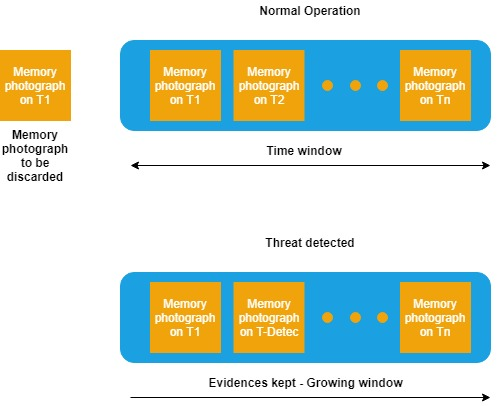
\includegraphics[scale=0.40]{janela_ieee-eng.jpg}
\centering
\label{fig:janela}
\end{figure}



\subsection{Secure data storage}
\label{sec:proposal-desc-memcpy}


%Aiming to persist the evidence-origin relationship, as well as to guarantee data integrity, \fancyname\ calculates the hash of the pair \{evidence, container image identifier\} and stores the triple \{hash, container image identifier, evidence\}.
%
Aiming to persist the evidence-origin relationship, as well as to guarantee data integrity, \fancyname\ calculates the hash $H$ of the pair \{memory photograph, resource identifier\} and stores the triple \{$H$, memory photograph, resource identifier\}.
%
The place of storage should be defined by the client and the cloud provider, and included in a service-level agreement (SLA).
%
If such SLA dictates that evidences must be stored outside the cloud environment, it is important to have the data transported using a secure channel (e.g. via \textit{Transport Layer Security} – TLS \cite{DierksT2008}).

%avoid possible problems with the storage of these data in countries with different jurisdictions from those in which they must be applied in the investigation in question, the evidence collected is stored in a physical place outside the cloud, after being transported by a secure channel (e.g. via \textit{Transport Layer Security} – TLS \cite{DierksT2008}).



\section{Experimental analysis}
\label{sec:proposal-impl}

\begin{figure}[htb!]
\footnotesize
\caption{\fancyname's general architecture. \marcos{Não precisa copiar 3x os mesmos blocos para explicar a solução... 1x basta... E por favor (1) aumente a fonte do texto na figura e (2) crie uma imagem vetorizada em pdf (e.g., no Visio dá para exportar como pdf)}}
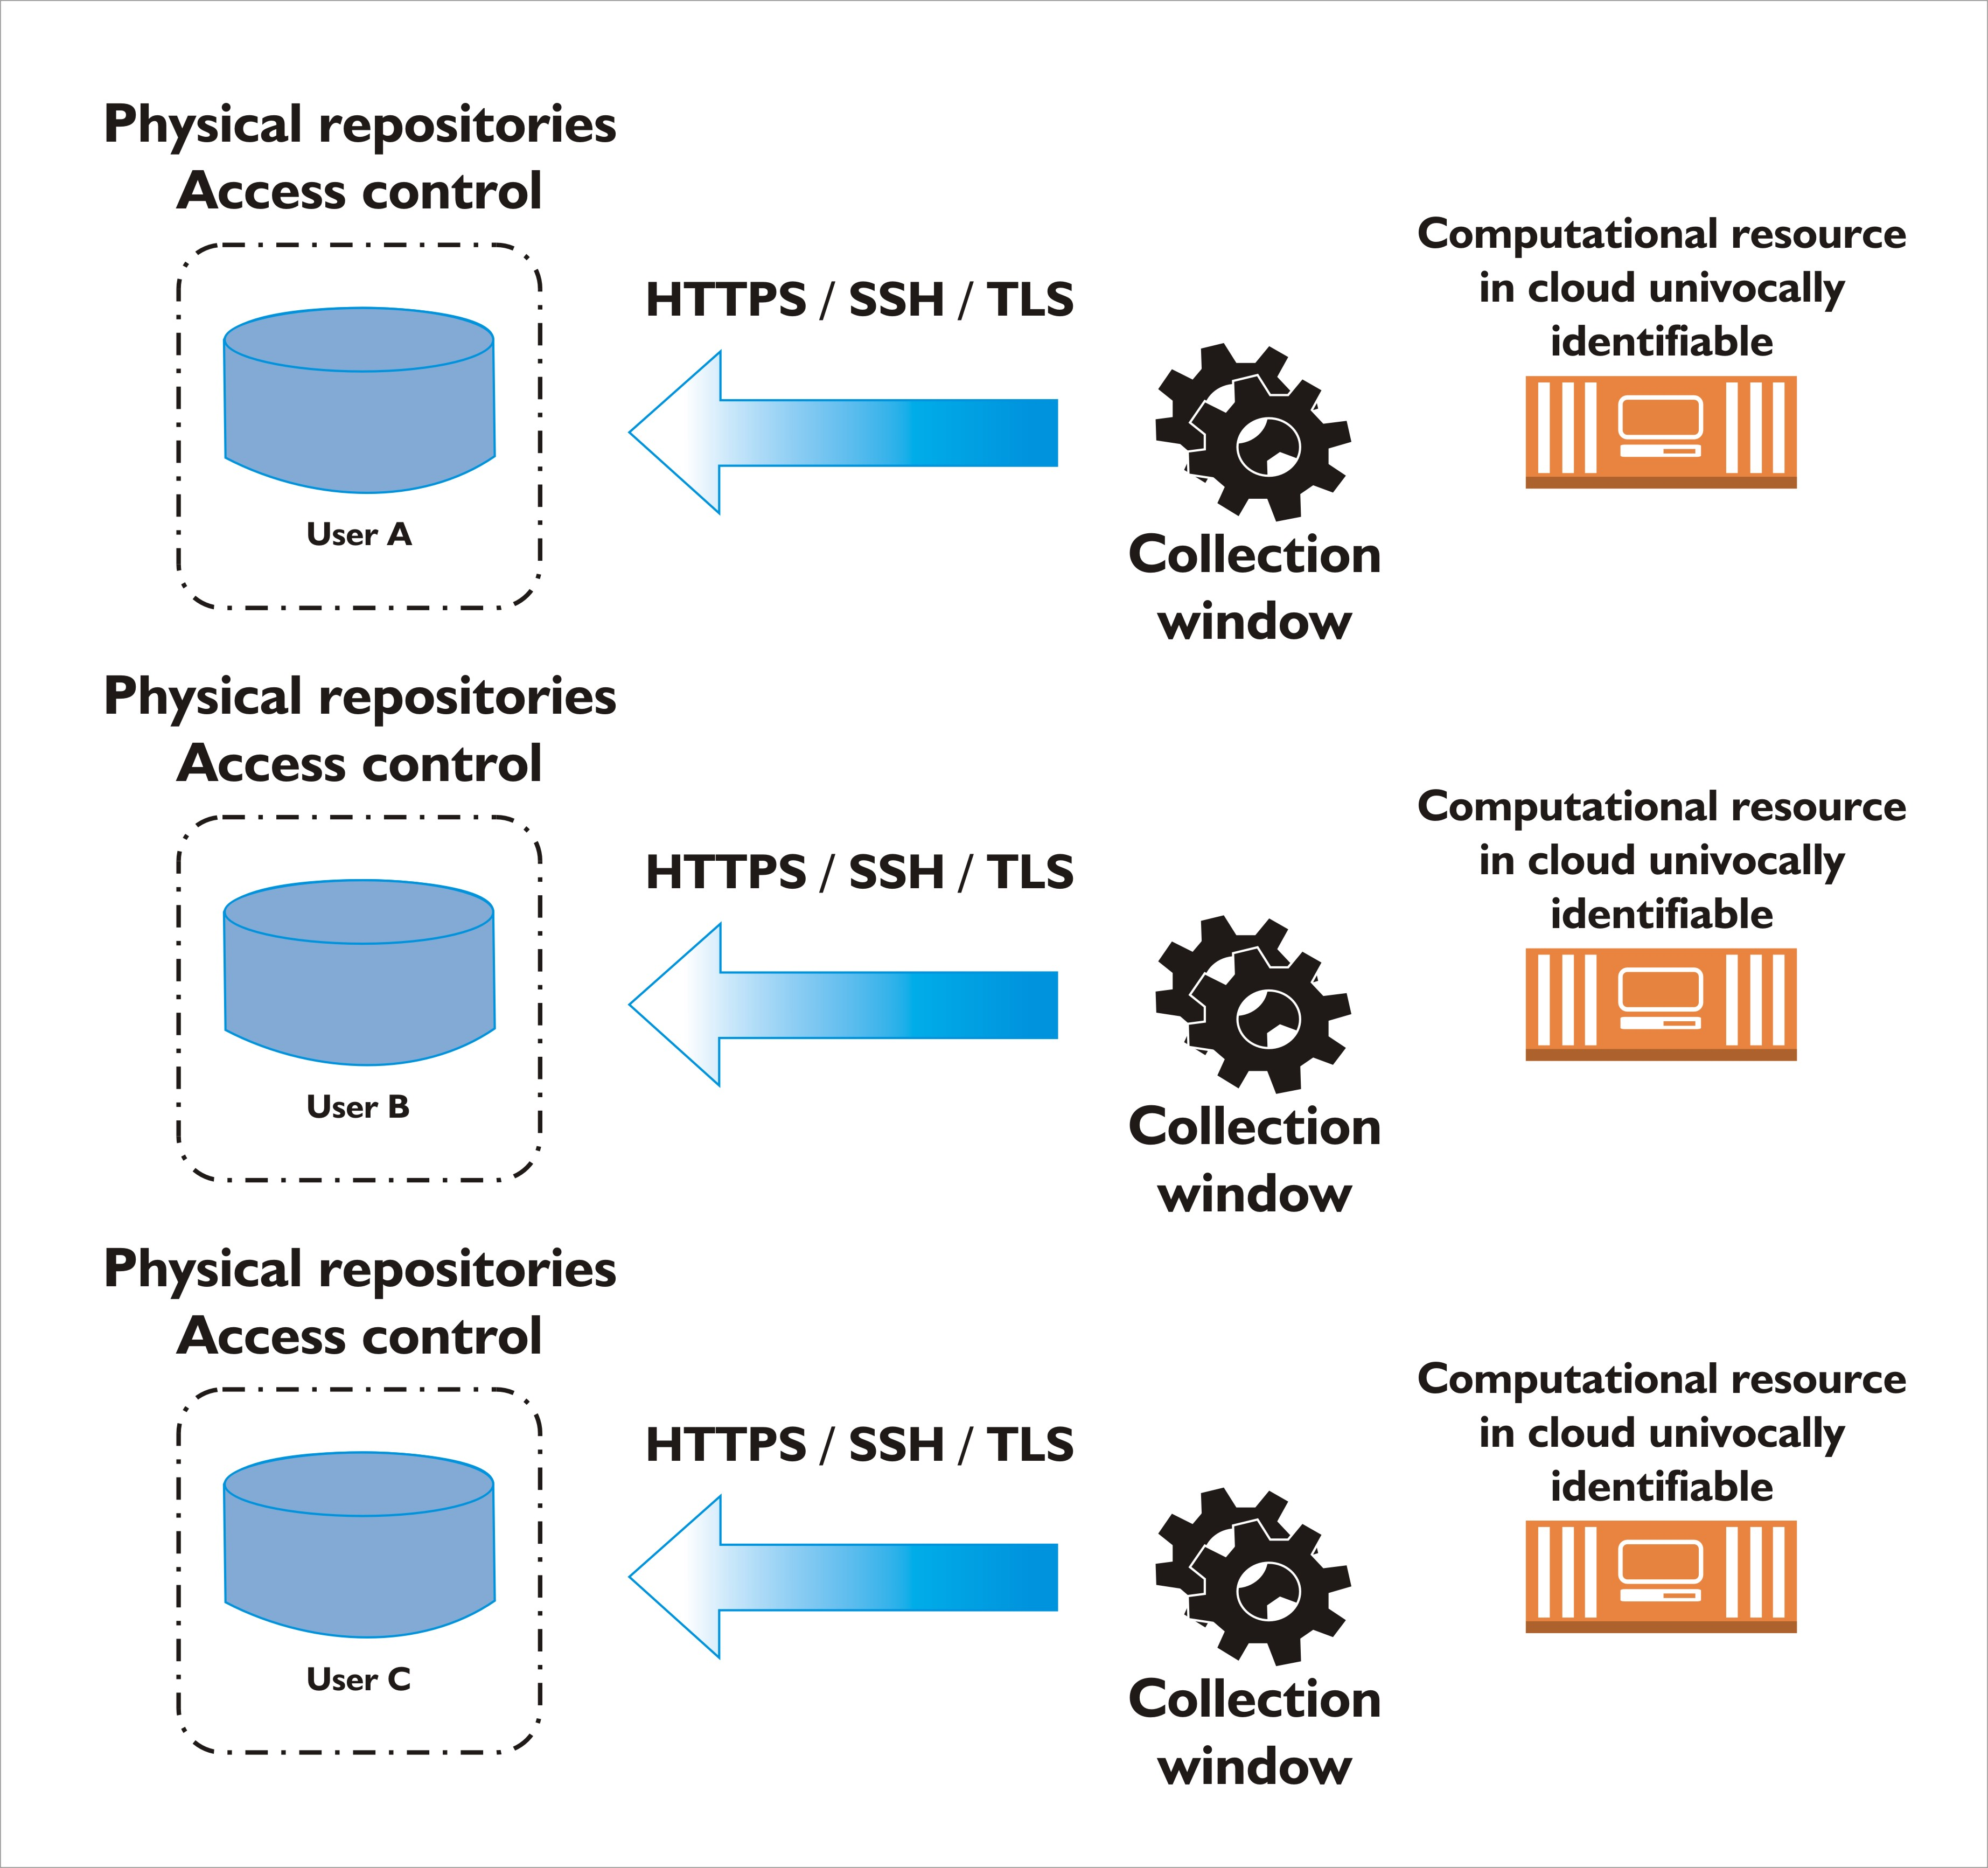
\includegraphics[scale=0.28]{solucao-eng.jpg}
\centering
\label{fig:Solucao}
\end{figure}


The \fancyname\ architecture was implemented in a testing platform, aiming to assess its efficacy and efficiency.
%in collecting the memory information from containers
%
The testbed employed, illustrated in Fig. \ref{fig:Solucao}, consists in creating a t2.micro instance (3.3 Mhz, 1GiB RAM and Linux 64-bit) at Amazon Web Services (AWS).
%
In this AWS instance, we installed Docker Engine 1.10 and API Docker 1.21, and then created 3 containers for executing the nginx 1.0 web server in different ports. 
%
Using a Java application that discovers the process identifier associated to each container \marcos{o que seria essa ``a Java application''? Você que desenvolveu? Tem que deixar claro se você usou algo ou desenvolveu esse algo}, we accessed the content \marcos{of that container's (é isso mesmo?? É do container ou é do sistema como um todo?)} \textit{Non-Uniform Memory Allocation descriptor} (\textbf{/proc/pid/numa\_maps}), containing the allocation of the memory pages, the nodes associated to these pages and what was allocated in their respective access policies \cite{UnixManPages_numa_maps}.
%
The copy and recording of the file is such that, every minute, the application (1) pauses the container in question, (2) copies the \textbf{numa\_maps} directory, (3) concatenates the data obtained with the container's image identifier, (4) calculates the hash $H$ for this set, and (5) saves the result in a \textbf{.mem} file named after the container's identifier.


The secure transportation of the evidence to a physical storage outside AWS employs another t2.micro instance, whereby an OpenVPN server is installed.
%
As a basic form of access control, the EC2 instance containing the evidence is configured to accept connections solely from machines in the VPN.
%
A physical machine outside AWS then uses an OpenVPN client to establish a VPN connection with the instance containing the evidence, obtaining the corresponding data.
%
After concluding the data acquisition process, the physical machine verifies whether there are local .mem files that older than a certain time interval, and discards them.


Using this testbed, two experiments were performed: the first focus on performance aspects, whereas the second evaluates \fancyname's ability to aid in identifying malware injection attacks.
%
Both experiments are described in the following sub-sections.

\subsection{Performance}
\label{sec:proposal-exp}

%To assess the \fancyname efficacy in collecting evidence, \textcolor{blue}{two experiments} were performed using the environment implemented (described in Section \ref{sec:proposal-impl}).
%
For the first experiment, the system was configured to collect memory photographs in 1-minute intervals and send them to the physical machine outside the cloud.
%
The data collection time window was set to 5 minutes, meaning that samples older than that are erased from the physical machine's disk.
%
The system was then executed for 30 minutes, and the following metrics were collected: 
(1) the disks space required for storing the memory photographs; 
(2) the time necessary for pausing a container and copying its contents; and 
(3) the time taken for transporting the evidence to the physical machine outside the cloud.
%
%After each data collection, the \textit{Unix} command \texttt{du -sh *.mem} was executed in the physical machine outside the cloud to return the list of the files in which the memory photographs were stored and the disk space they occupied. \marcos{fica repetitivo com o que já foi falado e com o que é falado na sequência}
%


The disk space occupied by the memory photographs captured during the experiment, obtained via the \textit{Unix} command \texttt{du -sh *.mem}, is shown in Fig. \ref{fig:evolucao_coleta}. 
%
This figure shows that, as expected, the disk space usage increases linearly until the time window is reached, and then stays constant due to older samples being discarded \marcos{Qual o tamanho de 1 sample? Essa info me parece relevante mencionar aqui}.
%
The discarding process can be halted at any time by the physical machine itself (e.g., after an attack is detected).
%
It is, thus, possible to describe the state of the system before and after an incident is detected, even after the corresponding cloud instances are erased.


%The solution thus keeps the disk space occupied by the samples collected under control.
%
%Concurrently, memory photographs saved by the solution after the containers and the AWS instance are removed and kept in the disk of the physical machine outside the cloud; they may be associated to their origin, as expected for a forensic analysis. 
%
%This ability is kept after a threat has been detected since, in this case, older collections stop being erased so it is possible to describe the state of the system before and after the incident \cite{Case_Memory_Forensics:2014}, allowing, for example, code injection attacks to the memory to be analyzed.


\begin{figure}[htb!]
\footnotesize
\caption{Evolution of disk space usage while running \fancyname.}
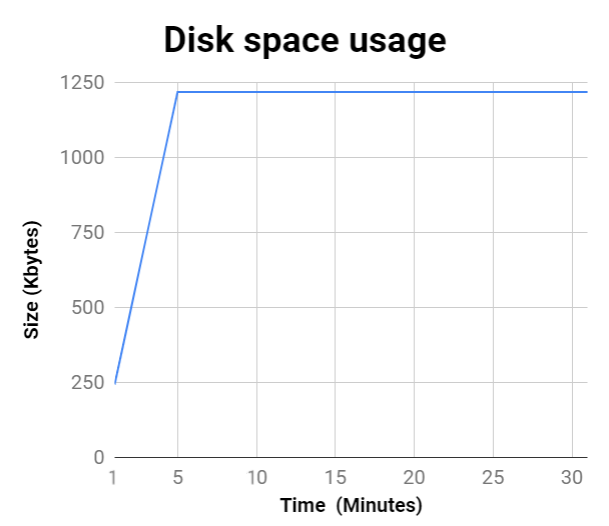
\includegraphics[scale=0.55]{evolucao_coleta_ieee.png}
\centering
\label{fig:evolucao_coleta}
\end{figure}


A potential issue of the proposed solution is that pausing a container to collect data may, at least in principle, cause efficiency losses of the application being executed.
%
To assess this overhead, the times for copying the container memory were measured along the experiment.
%
The results are shown in Figure \ref{fig:memoria_copia}.
%
Note that, after the application is initialized \marcos{O que você quer dizer com ``after the application is initialized''? Qual application (Dizang? WebServer? Outro?)? Aliás, se remover esse pedaço da sentença dá na mesma não? Enfim, é lógico que o tempo para fazer a cópia é medido depois de inicializado o processo de cópia (donde a dúvida de qual é a ``aplicação'' que você menciona)}, the time for making a copy is quite short, varying between 20 and 40 milliseconds. 
%
Especially for containers executing the engine of dynamic web pages, as is the case of the experiment in question, this latency can be not very perceptible by end users.
%
\textcolor{blue}{For the cases in which the interruption of the computational resource's execution for a short time causes problems of availability, it is possible to perform the collection procedure in separate moments of time. 
%
Thus, instead of suspending the execution of all computational resources to carry out the collection simultaneously, the procedure interrupts them sequentially.}
%
\marcos{Você quer dizer que aproveitaria o load-balancing e pararia 1 instância das 3 a cada instante, em round-robin? Eu entendi isso do texto, mas não ficou 100\% claro se é isso mesmo}

\begin{figure}[tb!]
\footnotesize
\caption{Time for copying the container \marcos{Aqui é ``median'' (=mediana) mesmo, ou é ``average'' (=média)? São duas coisas diferentes do ponto de vista de estatística}.}
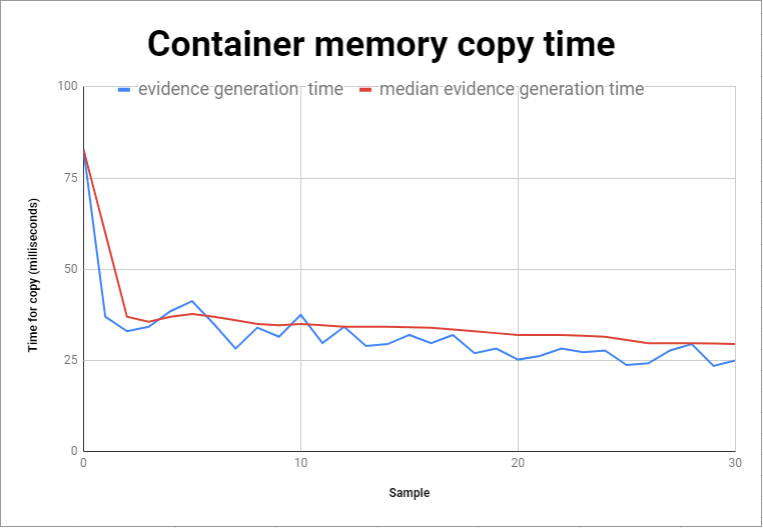
\includegraphics[scale=0.44]{memoria_copia_ieee.png}
\centering
\label{fig:memoria_copia}
\end{figure}


Another concern is the time for transporting the evidence to the storage outside the cloud.
%
The evidence transport to the storage outside the cloud can take longer than generation interval, leading to evidence loss during transport. 
%
To assess this impact, the evidence transport times for storage outside the cloud were measured along the experiment, as shown by the results in the graph of Fig. \ref{fig:evidencia_transporte}.
%
The transport time is verified to stabilize after the window size is reached. 
%
The time for transporting evidence is approximately 30 seconds on average. 
%
The topology is a factor that may contribute both positively and negatively to the transport time. 
%
In this experiment, the evidence generator is in North America, whereas the physical machine where the evidence was transported to is in South America.

\begin{figure}[htb!]
\footnotesize
\caption{Evidence transport time}
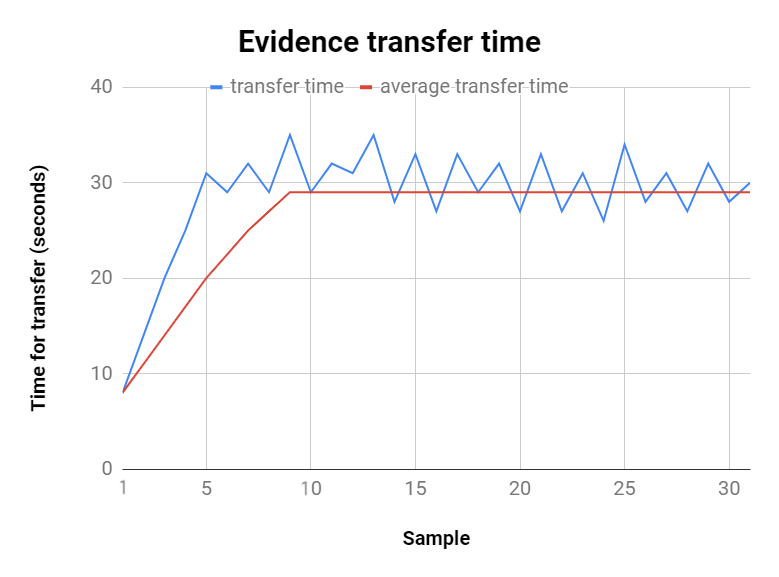
\includegraphics[scale=0.43]{evidencia_download_ieee.png}
\centering
\label{fig:evidencia_transporte}
\end{figure}


\textcolor{blue}{A second experiment aimed to determine if it is possible, through the analysis of the collected evidence, to identify malware injection in the container memory was made.
%
To this end, a library named \textbf{libexample.so} simulating a malware in the form of a library was injected into one of the containers.
%
After five minutes of \fancyname collecting evidence, the library mentioned berfore was injected into the memory of one of the containers. 
%
After the injection the solution was allowed to continue collecting memory snapshots for another 5 minutes.
%
In addition to collecting directory content \textbf{/proc/pid/numa\_maps}, a raw copy of the process memory of the container was also performed using the Linux \textit{GDB} utility via the command described in Figure \ref{fig:comando-copia}.}

\begin{figure*}[htb!]
\footnotesize
\caption{Command to generate a raw copy of the process container memory}
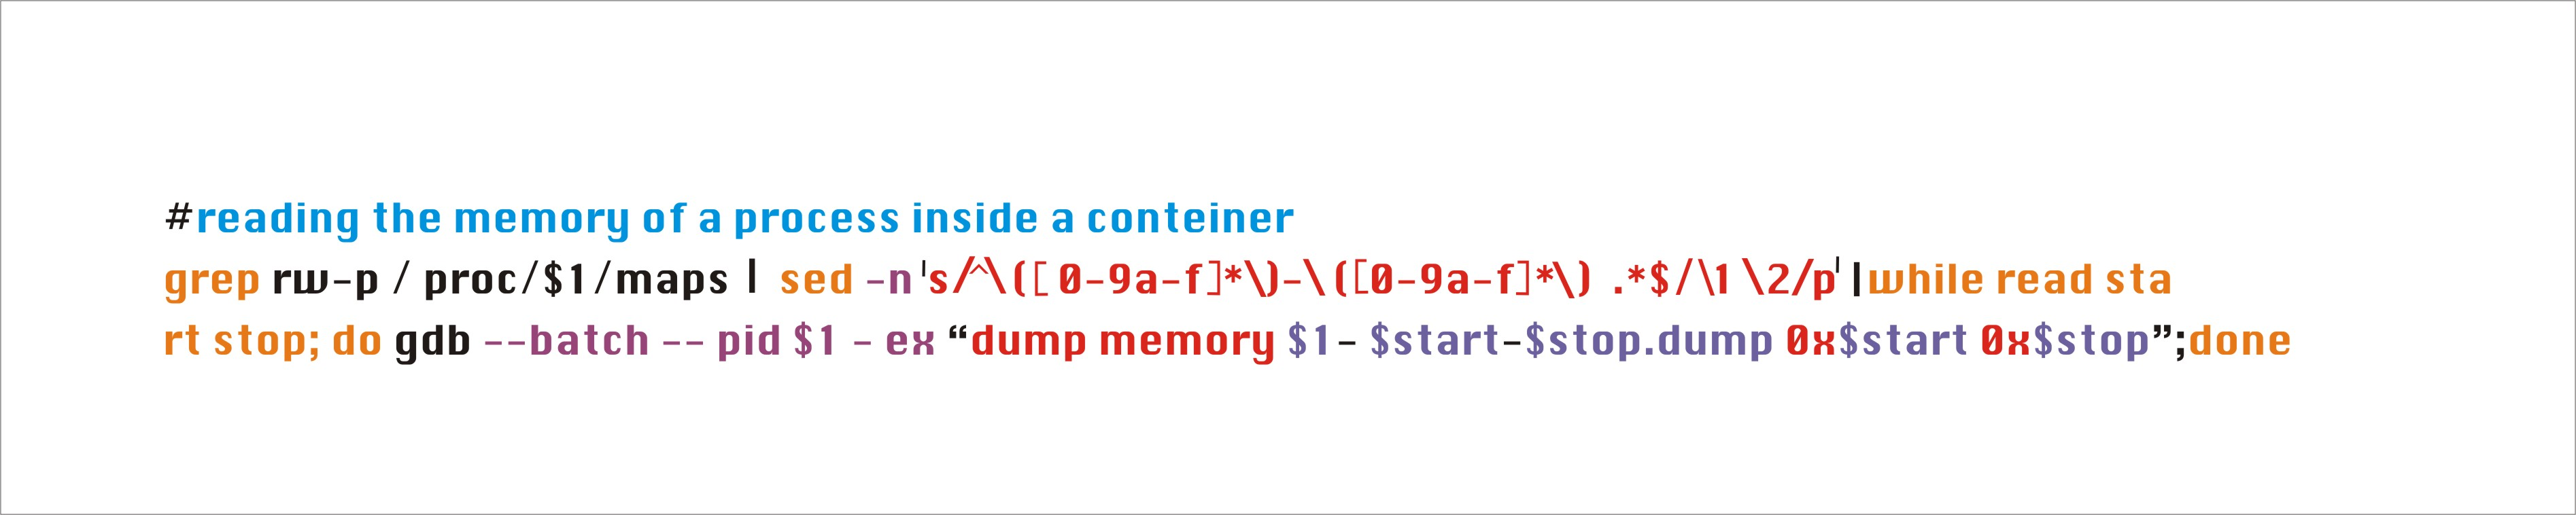
\includegraphics[scale=0.40]{comando-copia-memoria-gdb.jpg}
\centering
\label{fig:comando-copia}
\end{figure*}


\textcolor{blue}{Two distinct moments were compared in the life of the container, before and after the injection of the library.
%
Figure \ref{fig:antes-injecao} shows part of the memory before the injection and Figure \ref{fig:apos-injecao} shows part of the memory after the injection.
%
It is possible to see the injected \textbf{libexample.so} library between addresses \textbf{7fbb52a50000} and \textbf{7fbb52c51000} in the snapshot after the injection.
%
Therefore, it is possible to identify the injection of a malware in the form of a library via evidence collected by \fancyname from the \textbf{/proc/pid/numa\_maps} directory via comparison between two memory snapshots.
%
This allows code injection attacks to be identified.}

\begin{figure}[htb!]
\footnotesize
\caption{Part of \textbf{/proc/pid/numa\_maps} file BEFORE injection }
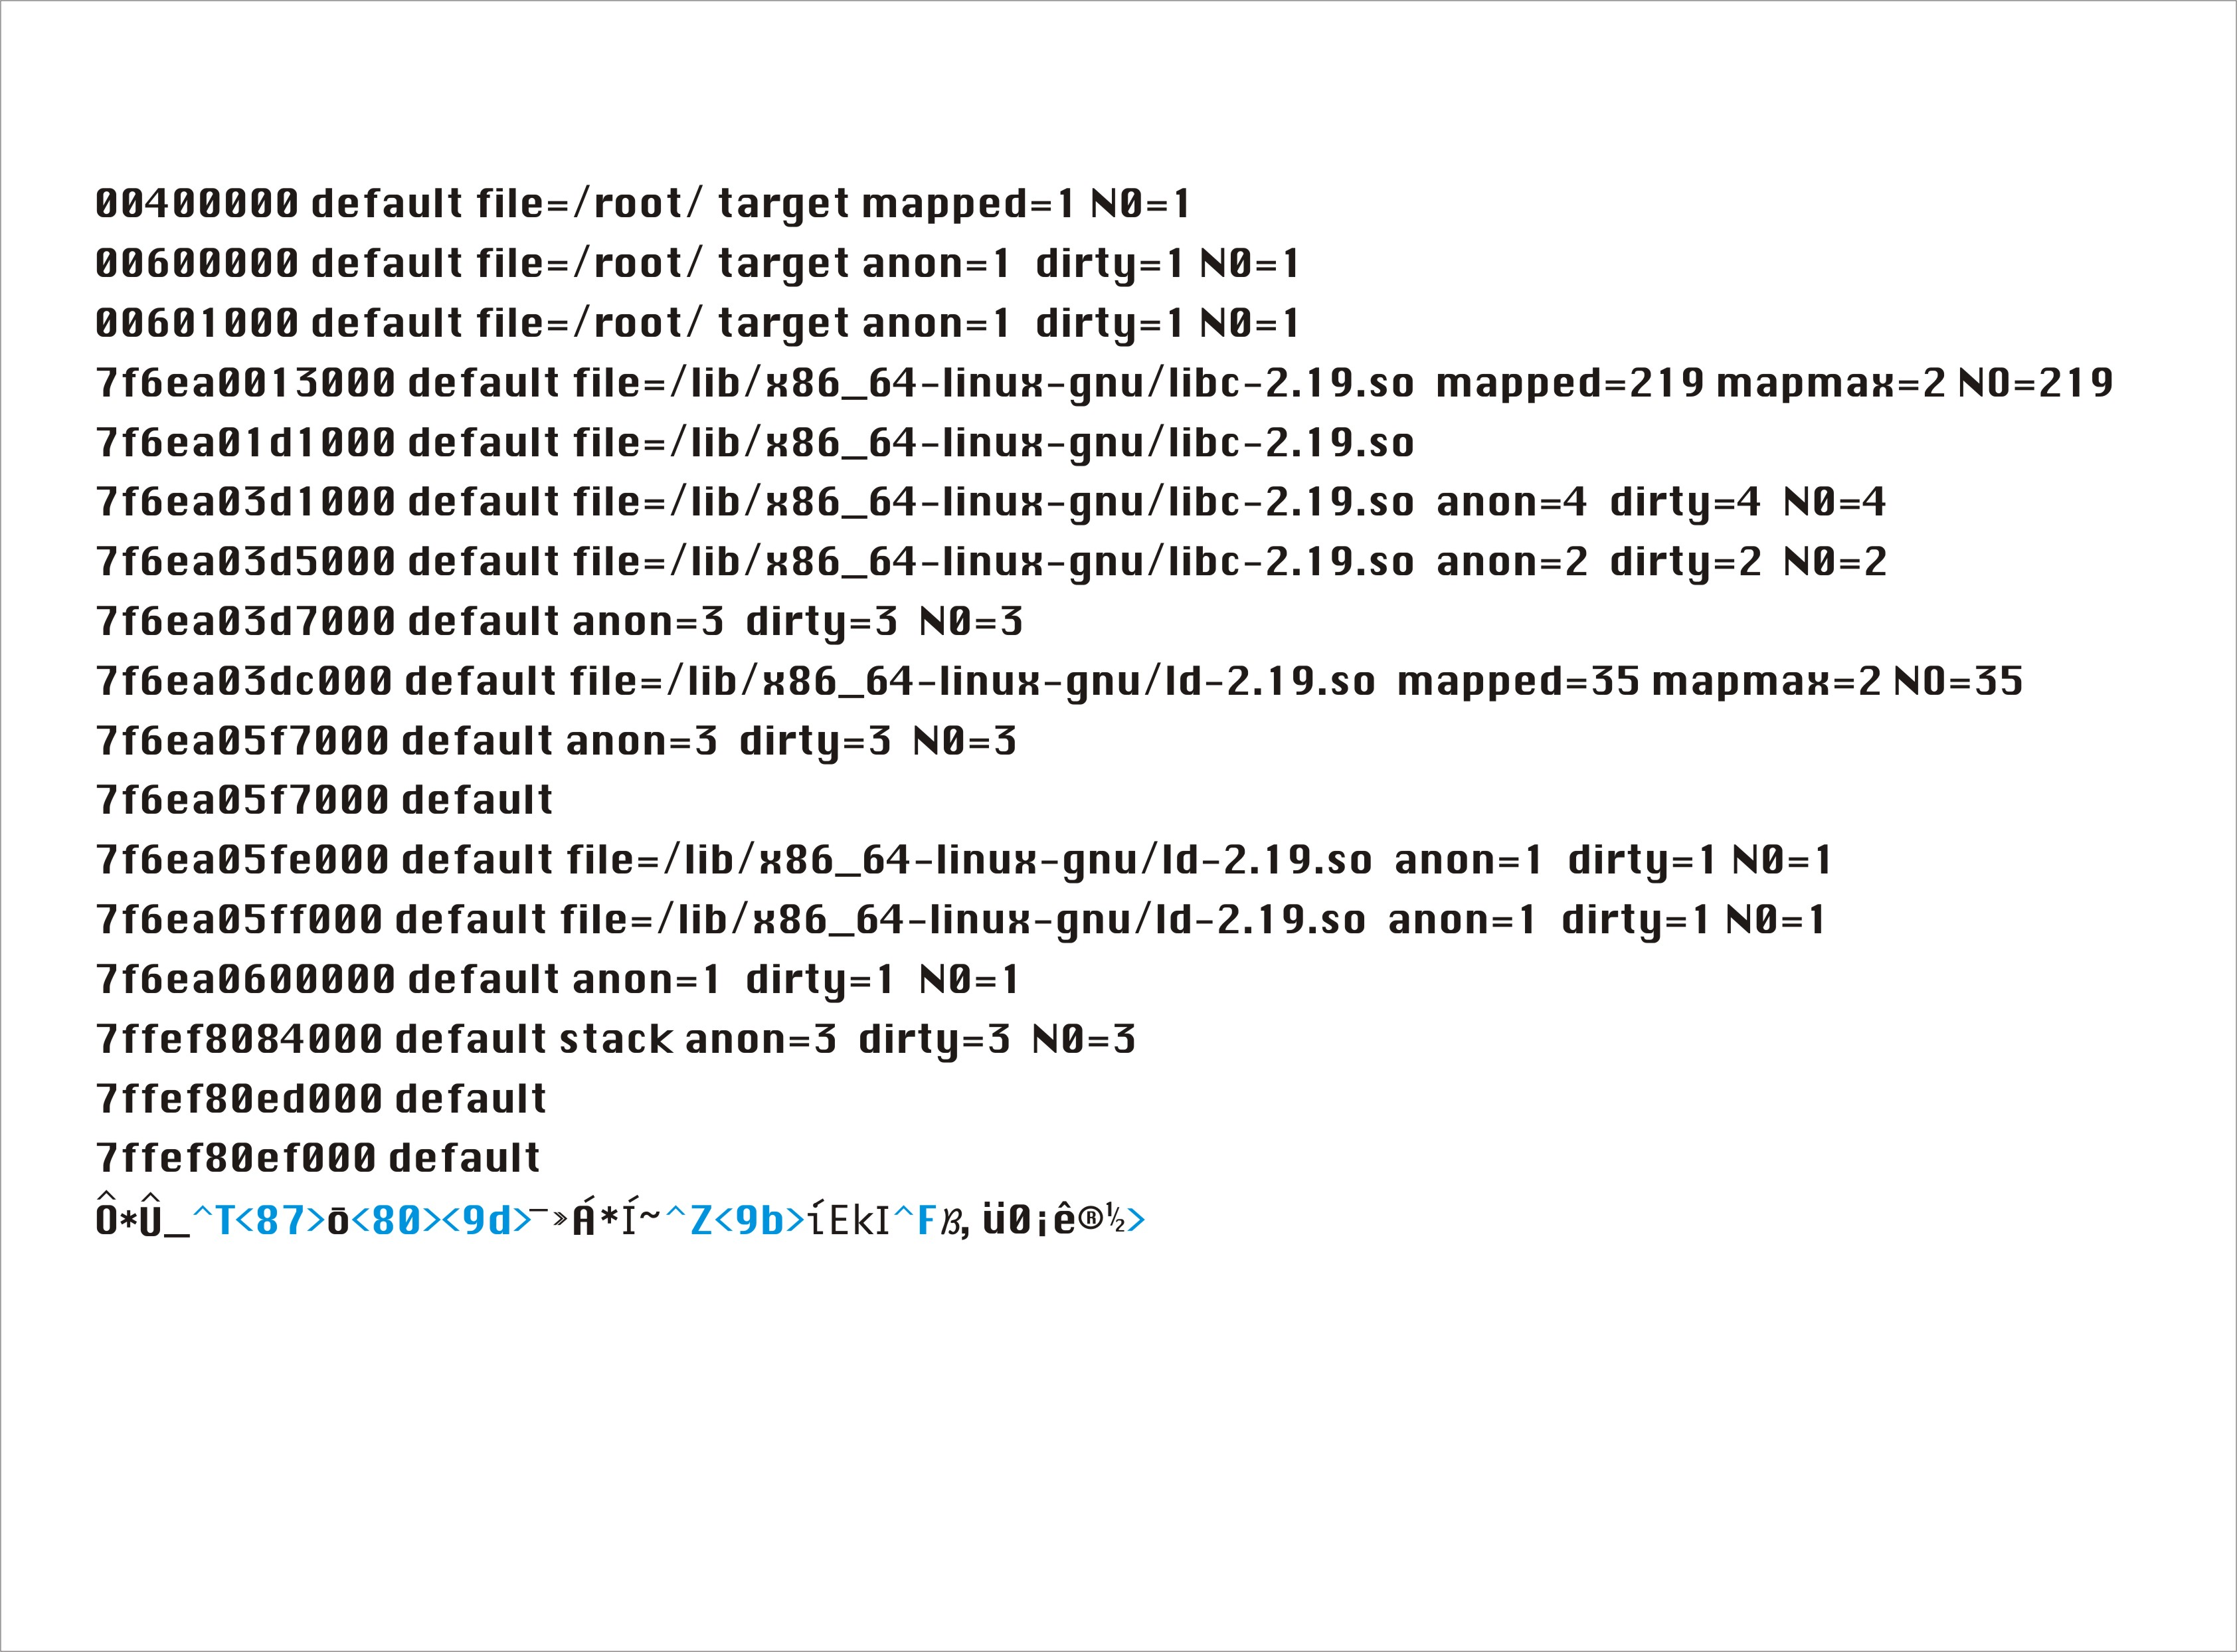
\includegraphics[scale=0.31]{antes-injecao.jpg}
\centering
\label{fig:antes-injecao}
\end{figure}


\begin{figure}[htb!]
\footnotesize
\caption{Part of \textbf{/proc/pid/numa\_maps} file AFTER injection }
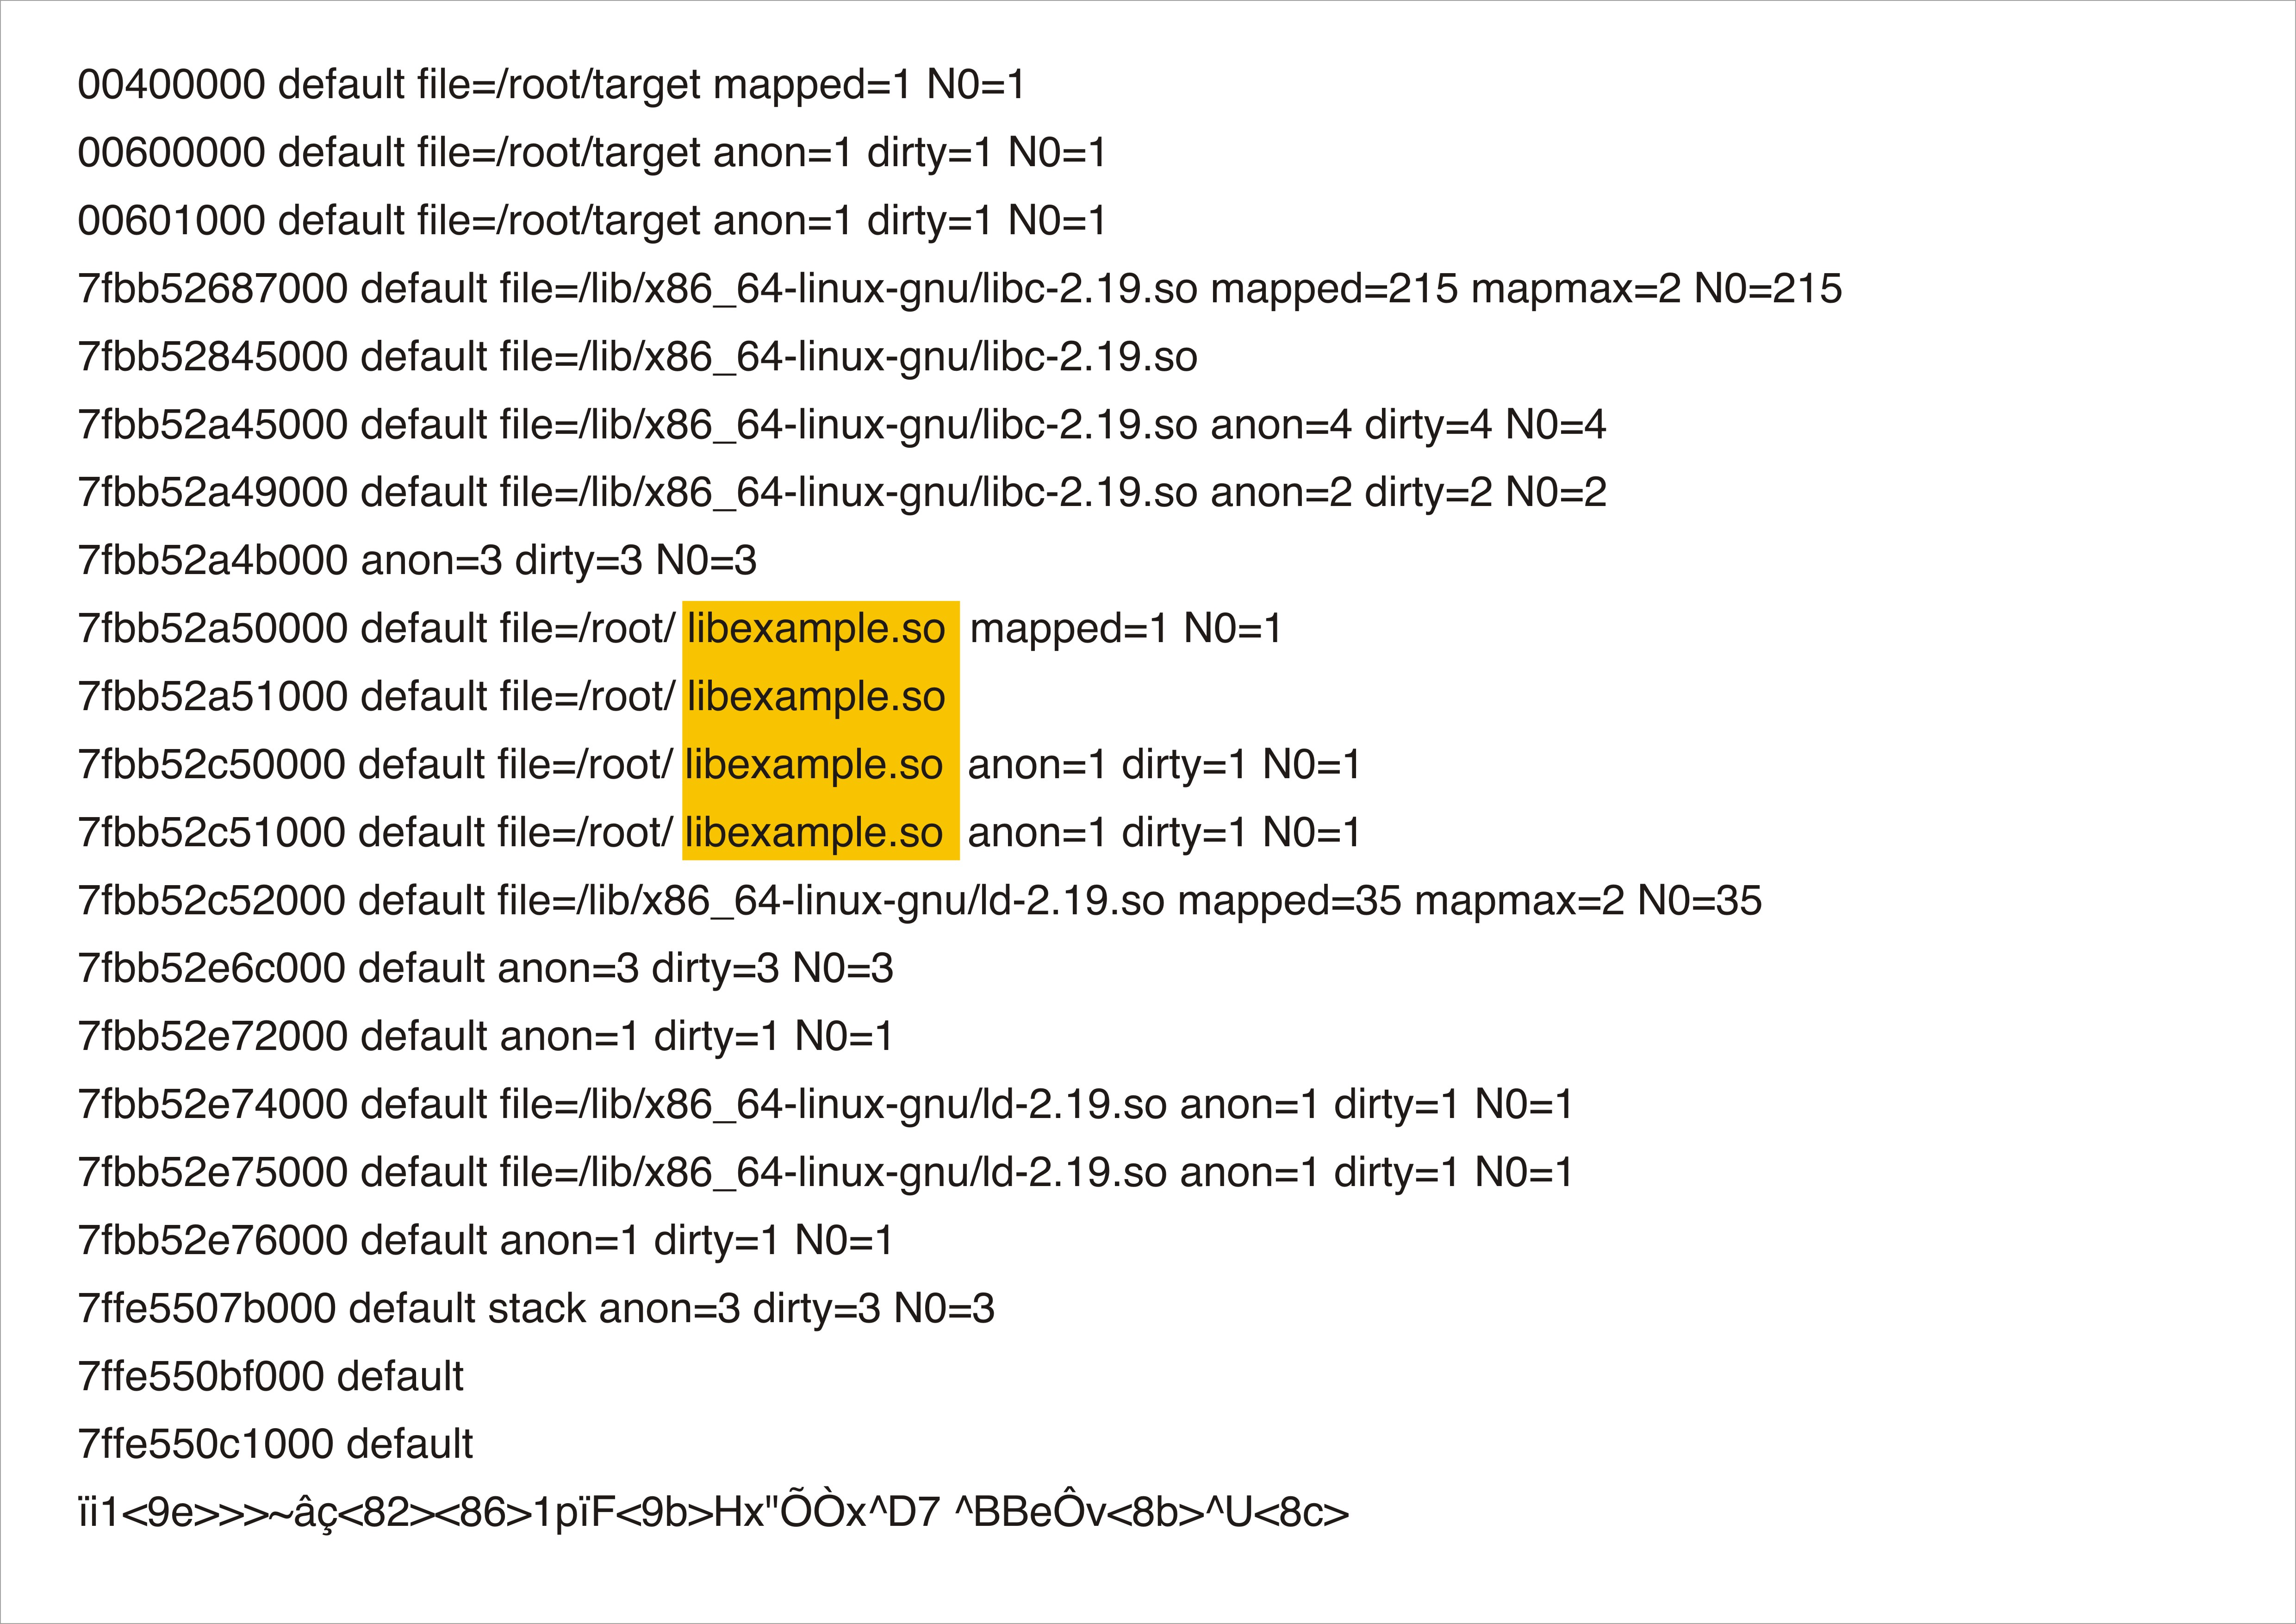
\includegraphics[scale=0.21]{apos-injecao.jpg}
\centering
\label{fig:apos-injecao}
\end{figure}


\textcolor{blue}{Despite the successful collection by copying the \textbf{/proc/pid/numa\_maps}, it was not possible to copy the contents of the process memory from the container via \textit{ptrace}.
%
According to \cite{cgroupsxptrace}, this happens because the system calls used by tools such as \textit{ptrace} and \textit{htop} were created before the implementation of \textit{cgroups} in the linux \textit{kernel} and thus are not aware of the existence of isolation between processes.
%
When \textit{ptrace} tries to access an area of memory isolated by \textit{cgroups}, the kernel sends a memory access violation signal, the result is shown in Figure \ref{fig:erro-copia-gdb}.
%
The Docker Engine \cite{capabilities} documentation mentions the command \texttt{--cap-add=SYS\_PTRACE --security-opt-seccomp=unconfined} which allows \textit{ptrace} to access the memory of a process inside the container but does not allow the host machine or other container to access it.
%
Still according to \cite{cgroupsxptrace} an alternative to enable the monitoring and access to memory information would be to expose such information in the structure of \textbf{/sys/fs/cgroup/} in the same way that it is made to \textbf{/proc/pid/}.}

\begin{figure}[htb!]
\footnotesize
\caption{Error while attempting to copy the memory of a process inside a container}
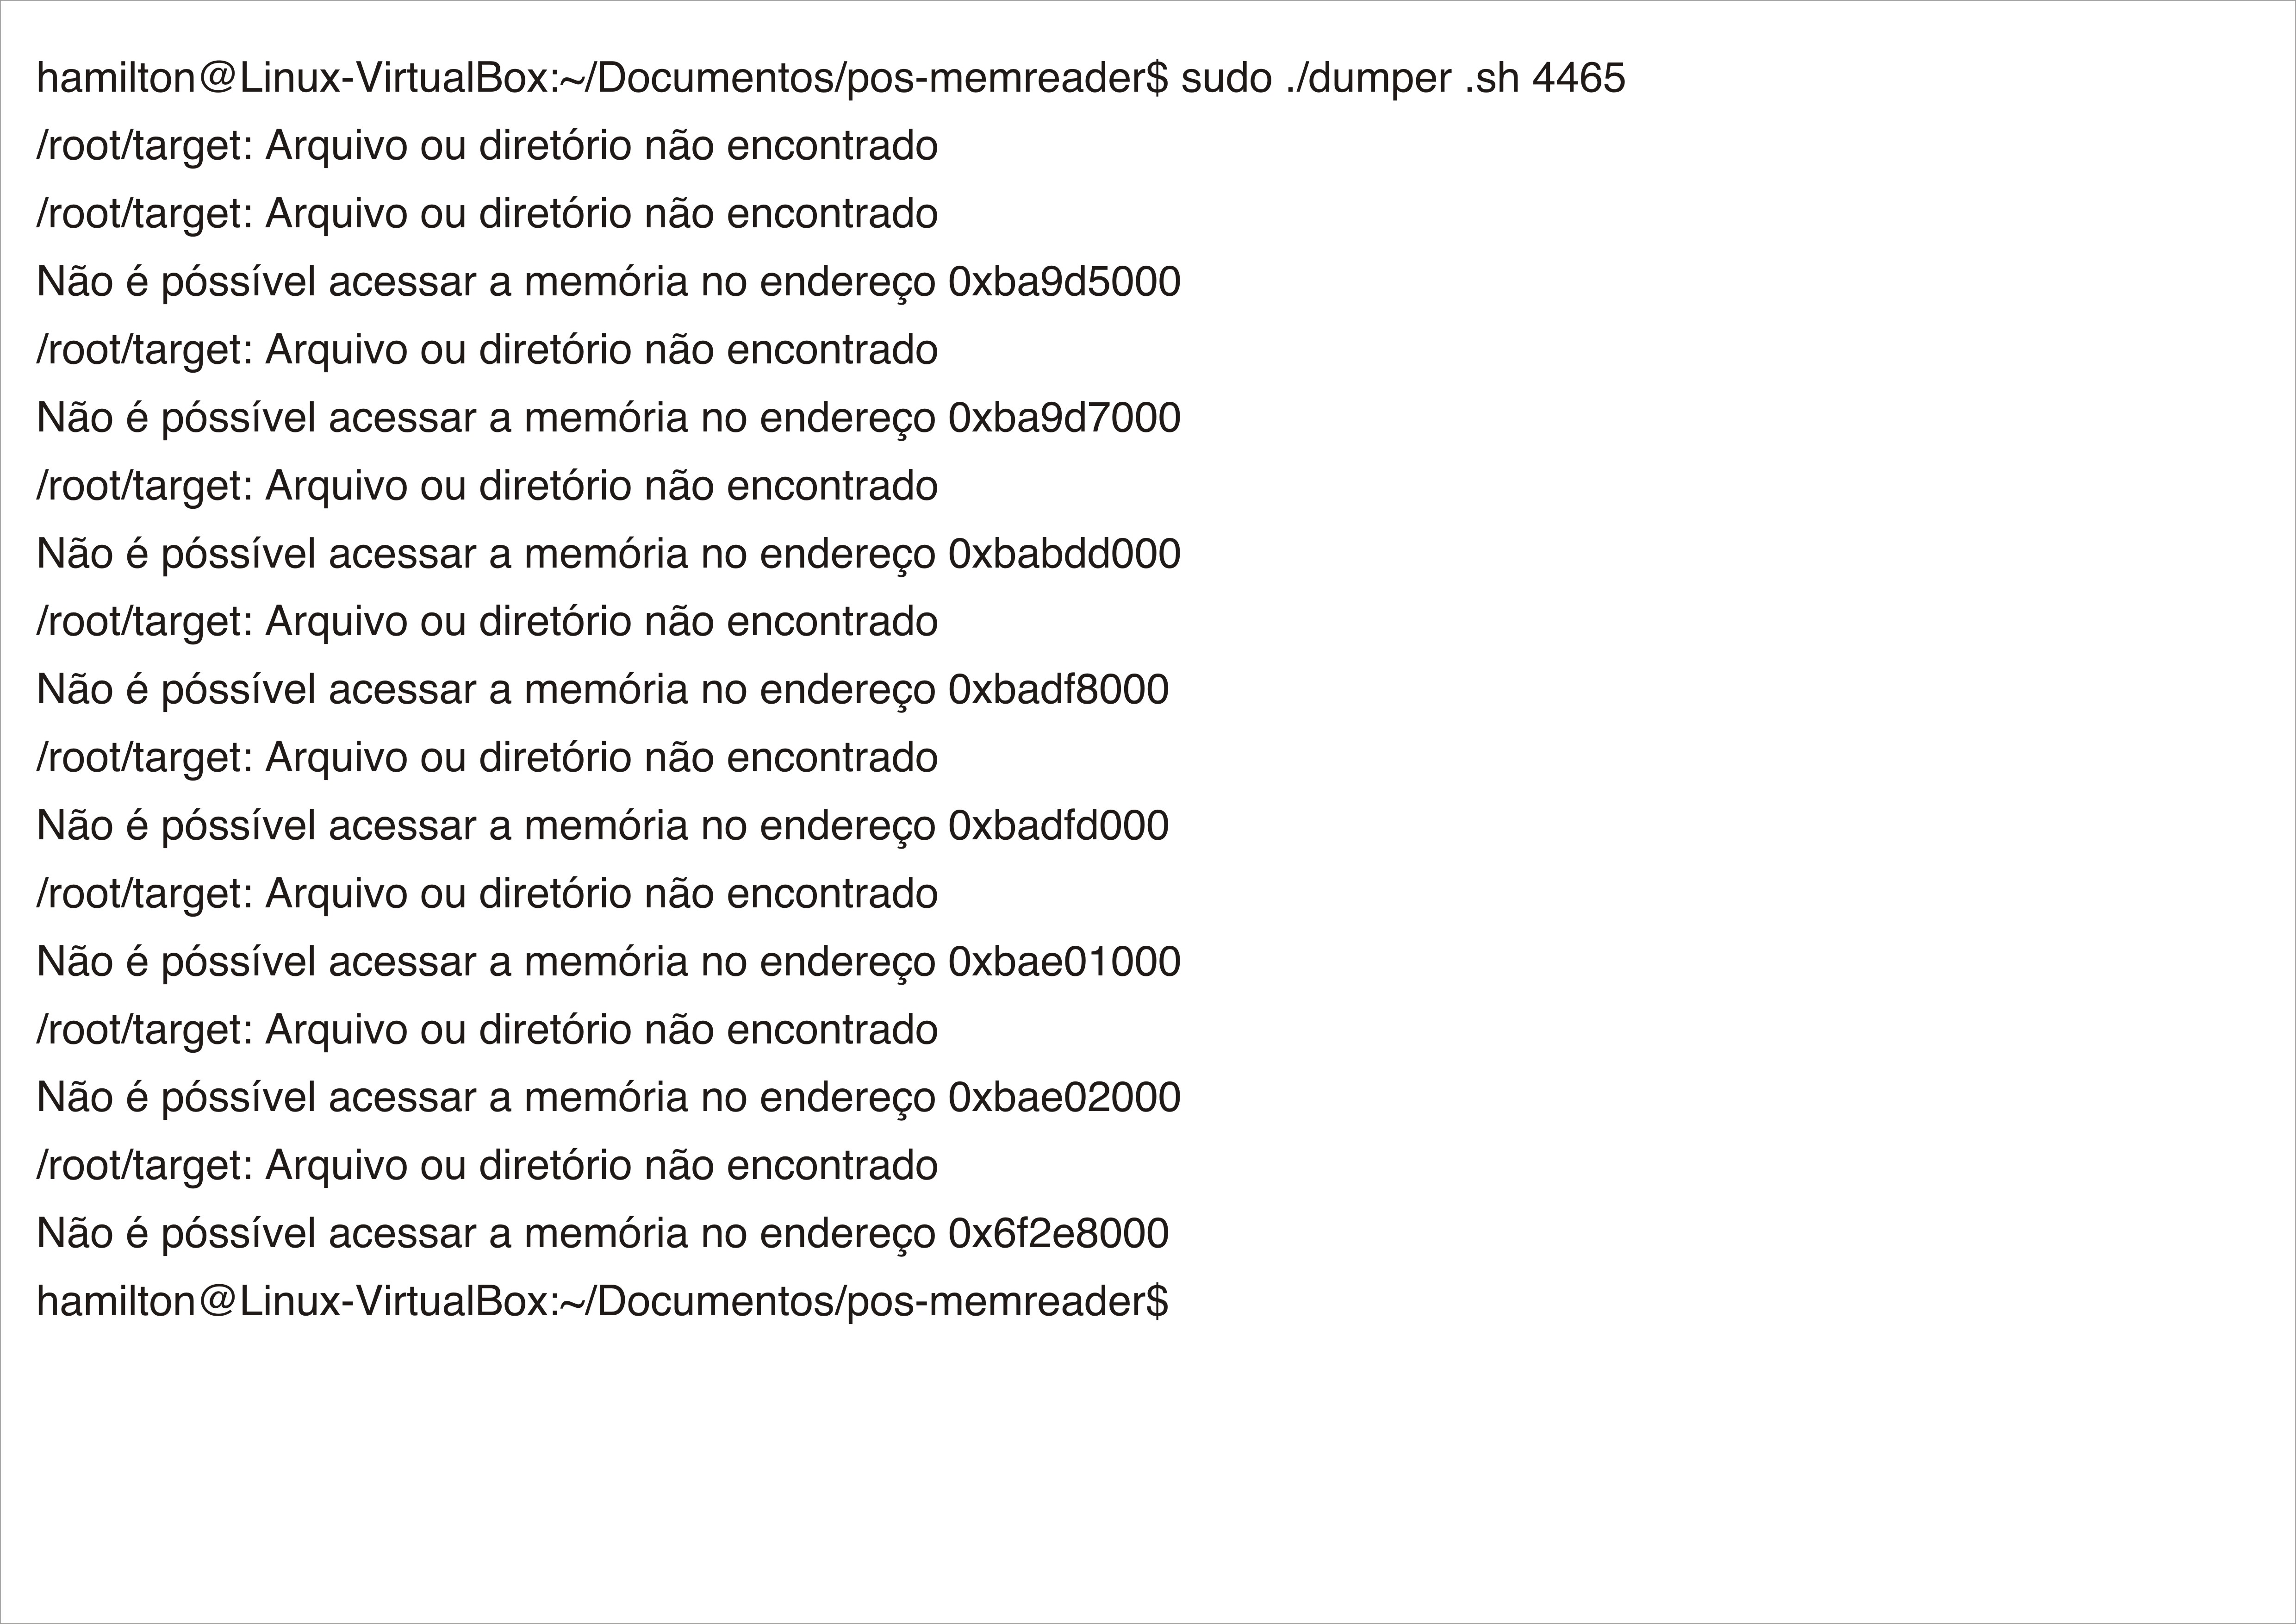
\includegraphics[scale=0.21]{nao-consido-dumpar-memoria.jpg}
\centering
\label{fig:erro-copia-gdb}
\end{figure}


\subsection{Limitations}

\textcolor{blue}{The described proposal calls for the cloud resource to be uniquely identifiable in order to make the association between evidence and its origin.
%
During the course of this project this unique form of identification was only possible through the hash of the container image. This was the only feature that, submitted to the build process from the same recipe resulted in the same hash of the image.
%
So, the implementation for validating the proposed solution can only collect memory information in \textit{user space}.
%
In principle, therefore, \fancyname does not provide support to malware investigation techniques based on information from the kernel space, such as comparing the information from the \textit{Process Environment Block} (PEB), which are in the user space, with information from the \textit{Virtual Address Descriptor} (VAD), which lies in the kernel space. 
%
Analyses of threats that directly manipulate the objects of the kernel (D.K.O.M – \textit{Direct Kernel Object Manipulation}) do not benefit from the solution proposed, either.}


% An example of a floating figure using the graphicx package.
% Note that \label must occur AFTER (or within) \caption.
% For figures, \caption should occur after the \includegraphics.
% Note that IEEEtran v1.7 and later has special internal code that
% is designed to preserve the operation of \label within \caption
% even when the captionsoff option is in effect. However, because
% of issues like this, it may be the safest practice to put all your
% \label just after \caption rather than within \caption{}.
%
% Reminder: the "draftcls" or "draftclsnofoot", not "draft", class
% option should be used if it is desired that the figures are to be
% displayed while in draft mode.
%
%\begin{figure}[!t]
%\centering
%\includegraphics[width=2.5in]{myfigure}
% where an .eps filename suffix will be assumed under latex, 
% and a .pdf suffix will be assumed for pdflatex; or what has been declared
% via \DeclareGraphicsExtensions.
%\caption{Simulation Results.}
%\label{fig_sim}
%\end{figure}

% Note that IEEE typically puts floats only at the top, even when this
% results in a large percentage of a column being occupied by floats.


% An example of a double column floating figure using two subfigures.
% (The subfig.sty package must be loaded for this to work.)
% The subfigure \label commands are set within each subfloat command,
% and the \label for the overall figure must come after \caption.
% \hfil is used as a separator to get equal spacing.
% Watch out that the combined width of all the subfigures on a 
% line do not exceed the text width or a line break will occur.
%
%\begin{figure*}[!t]
%\centering
%\subfloat[Case I]{\includegraphics[width=2.5in]{box}%
%\label{fig_first_case}}
%\hfil
%\subfloat[Case II]{\includegraphics[width=2.5in]{box}%
%\label{fig_second_case}}
%\caption{Simulation results.}
%\label{fig_sim}
%\end{figure*}
%
% Note that often IEEE papers with subfigures do not employ subfigure
% captions (using the optional argument to \subfloat[]), but instead will
% reference/describe all of them (a), (b), etc., within the main caption.


% An example of a floating table. Note that, for IEEE style tables, the 
% \caption command should come BEFORE the table. Table text will default to
% \footnotesize as IEEE normally uses this smaller font for tables.
% The \label must come after \caption as always.
%
%\begin{table}[!t]
%% increase table row spacing, adjust to taste
%\renewcommand{\arraystretch}{1.3}
% if using array.sty, it might be a good idea to tweak the value of
% \extrarowheight as needed to properly center the text within the cells
%\caption{An Example of a Table}
%\label{table_example}
%\centering
%% Some packages, such as MDW tools, offer better commands for making tables
%% than the plain LaTeX2e tabular which is used here.
%\begin{tabular}{|c||c|}
%\hline
%One & Two\\
%\hline
%Three & Four\\
%\hline
%\end{tabular}
%\end{table}


% Note that IEEE does not put floats in the very first column - or typically
% anywhere on the first page for that matter. Also, in-text middle ("here")
% positioning is not used. Most IEEE journals/conferences use top floats
% exclusively. Note that, LaTeX2e, unlike IEEE journals/conferences, places
% footnotes above bottom floats. This can be corrected via the \fnbelowfloat
% command of the stfloats package.

\section{Final Considerations}
\label{sec:conclusion}

Digital threats acting directly on the system memory do not usually leave traces in disk after their corresponding resources are removed, hindering later forensic analyses.
%
This problem is especially notable in cloud computing systems, in which the allocation and removal of virtualized resources (e.g. VMs and containers) are frequent.
%
This characteristic, together with aspects such as multitenancy and multi-jurisdiction of computational clouds, hinders evidence collection for investigating incidents.


In this scenario, the proposal presented aims to relate the memory photograph to its origin, using the calculated hash of the container image as a stored evidence identifier.
%
To prevent an excessive use of disk space, the volume of data stored uses a storage window, which allows describing the memory before and after an attack (e.g. memory injection).
%
Combined with a tool for identifying threats, these \fancyname characteristics make it a robust solution to provide evidence and thus make forensic analyses in the cloud viable.
%

\textcolor{blue}{As mentioned before, it was not possible to copy the contents of the process running inside the container.
%
Due to the complexity and knowledge required to perform the suggested modification and the process for accepting it in the linux code base, it is recommended for future work to incorporate into \fancyname a way of solving access to the contents of the memory of a container from the host system.}



% trigger a \newpage just before the given reference
% number - used to balance the columns on the last page
% adjust value as needed - may need to be readjusted if
% the document is modified later
%\IEEEtriggeratref{8}
% The "triggered" command can be changed if desired:
%\IEEEtriggercmd{\enlargethispage{-5in}}

% references section

% can use a bibliography generated by BibTeX as a .bbl file
% BibTeX documentation can be easily obtained at:
% http://www.ctan.org/tex-archive/biblio/bibtex/contrib/doc/
% The IEEEtran BibTeX style support page is at:
% http://www.michaelshell.org/tex/ieeetran/bibtex/
\bibliographystyle{IEEEtran}
% argument is your BibTeX string definitions and bibliography database(s)
\bibliography{artigo-ieee}

% <OR> manually copy in the resultant .bbl file
% set second argument of \begin to the number of references
% (used to reserve space for the reference number labels box)

\end{document}


